\documentclass[10pt,letterpaper,cm]{nupset}
\usepackage[margin=1in]{geometry}
\usepackage{graphicx}
 \usepackage{enumerate}
  \usepackage{enumitem}
 \usepackage{stmaryrd}
\usepackage{amsfonts}
\usepackage{amssymb}
\usepackage{pgfplots}
\pgfplotsset{compat=1.13}
\usepackage{amsmath,amsthm}
\usepackage{lmodern}
\usepackage{tikz-cd}
\usetikzlibrary{automata,positioning}
\usetikzlibrary{quotes}
\usepackage{faktor}
\usepackage{xfrac}
\usepackage{mathtools}
\usepackage{bm}
\usepackage{xcolor}
\usepackage{soul}
\usepackage{ dsfont }
\usepackage{stackengine}
\usepackage{mathrsfs}
\usepackage{hyperref}
\usepackage[linesnumbered,ruled]{algorithm2e}
\hypersetup{colorlinks=true, linkcolor=red,          % color of internal links (change box color with linkbordercolor)
    citecolor=green,        % color of links to bibliography
    filecolor=magenta,      % color of file links
    urlcolor=cyan           }
\usepackage{thmtools}
\usepackage[capitalise]{cleveref} 
    
\theoremstyle{definition}
\newtheorem{definition}{Definition}[subsection]
\newtheorem{exmp}[definition]{Example}
\newtheorem{non-exmp}[definition]{Non-example}
\newtheorem{note}[definition]{Note}

\theoremstyle{theorem}
\newtheorem{theorem}[definition]{Theorem}
\newtheorem{lemma}[definition]{Lemma}
\newtheorem{prop}[definition]{Proposition}
\newtheorem{corollary}[definition]{Corollary}
\newtheorem*{claim}{Claim}
\newtheorem{exercise}[definition]{Exercise}

\theoremstyle{remark}
\newtheorem{remark}[definition]{Remark}
\newtheorem*{todo}{To do}
\newtheorem*{conv}{Convention}
\newtheorem*{aside}{Aside}
\newtheorem*{notation}{Notation}
\newtheorem*{term}{Terminology}
\newtheorem*{background}{Background}
\newtheorem*{further}{Further reading}
\newtheorem*{sources}{Sources}
\newtheorem*{prob}{Problem}

\makeatletter
\def\th@plain{%
  \thm@notefont{}% same as heading font
  \itshape % body font
}
\def\th@definition{%
  \thm@notefont{}% same as heading font
  \normalfont % body font
}
\makeatother


\makeatletter
\renewcommand*\env@matrix[1][*\c@MaxMatrixCols c]{%
  \hskip -\arraycolsep
  \let\@ifnextchar\new@ifnextchar
  \array{#1}}
\makeatother
\pgfplotsset{unit circle/.style={width=4cm,height=4cm,axis lines=middle,xtick=\empty,ytick=\empty,axis equal,enlargelimits,xmax=1,ymax=1,xmin=-1,ymin=-1,domain=0:pi/2}}

\def\ruleoffset{1pt}
\newcommand\specialvdash[2]{\mathrel{\ensurestackMath{
  \mkern2mu\rule[-\dp\strutbox]{.4pt}{\baselineskip}\stackon[\ruleoffset]{
    \stackunder[\dimexpr\ruleoffset-.4\ht\strutbox+.4\dp\strutbox]{
      \rule[\dimexpr.4\ht\strutbox-.4\dp\strutbox]{2.5ex}{.4pt}}{
        \scriptstyle #1}}{\scriptstyle#2}\mkern2mu}}
}

\newcommand{\A}{\mathcal A}
\newcommand{\C}{\mathbb C}
\newcommand{\E}{\vec E}
\newcommand{\CP}{\mathbb CP}
\newcommand{\F}{\mathbb F}
\newcommand{\G}{\mathbb G}
\renewcommand{\H}{\mathcal H}
\newcommand{\HP}{\mathbb HP}
\newcommand{\K}{\mathbb K}
\renewcommand{\L}{\mathcal L}
\newcommand{\M}{\mathbb M}
\newcommand{\N}{\mathbb N}
\renewcommand{\O}{\mathbf O}
\newcommand{\OP}{\mathbb OP}
\renewcommand{\P}{\mathcal P}
\newcommand{\Q}{\mathbb Q}
\newcommand{\I}{\mathbb I}
\newcommand{\R}{\mathbb R}
\newcommand{\RP}{\mathbb RP}
\renewcommand{\S}{\mathbf S}
\newcommand{\T}{\mathbf T}
\newcommand{\Z}{\mathbb Z}
\newcommand{\B}{\mathcal{B}}
\newcommand{\1}{\mathbf{1}}
\newcommand{\ds}{\displaystyle}
\newcommand{\ran}{\right>}
\newcommand{\lan}{\left<}
\newcommand{\bmat}[1]{\begin{bmatrix} #1 \end{bmatrix}}

\renewcommand{\a}{\mathscr{A}}
\renewcommand{\b}{\mathscr{B}}
\renewcommand{\c}{\mathscr{C}}
\renewcommand{\d}{\mathscr{D}}
\newcommand{\e}{\mathscr{E}}
\newcommand{\y}{\mathscr{Y}}
\renewcommand{\j}{\mathscr{J}}
\newcommand{\X}{\mathscr X}
\newcommand{\accpt}{\mathrm{accpt}}
\newcommand{\h}{\vec h}
\newcommand{\f}{\vec f}
\newcommand{\g}{\vec g}
\renewcommand{\i}{\vec i}
\renewcommand{\k}{\vec k}
\newcommand{\n}{\vec n}
\newcommand{\p}{\vec p}
\newcommand{\q}{\vec q}
\renewcommand{\r}{\vec r}
\newcommand{\s}{\vec s}
\renewcommand{\t}{\vec t}
\renewcommand{\u}{\vec u}
\renewcommand{\v}{\vec v}
\newcommand{\w}{\vec w}
\newcommand{\x}{\vec x}
\newcommand{\z}{\vec z}
\newcommand{\0}{\vec 0}

\makeatletter
\newcommand*\bigcdot{\mathpalette\bigcdot@{.5}}
\newcommand*\bigcdot@[2]{\mathbin{\vcenter{\hbox{\scalebox{#2}{$\m@th#1\bullet$}}}}}
\makeatother

\DeclareMathOperator{\Ima}{Im}
\DeclareMathOperator*{\Span}{span}
\DeclareMathOperator*{\GL}{GL}
\DeclareMathOperator*{\SL}{SL}
\DeclareMathOperator{\rng}{range}
\DeclareMathOperator{\gemu}{gemu}
\DeclareMathOperator{\almu}{almu}
\newcommand{\Char}{\mathsf{char}}
\DeclareMathOperator{\id}{id}
\DeclareMathOperator{\graph}{Graph}
\DeclareMathOperator{\gal}{Gal}
\DeclareMathOperator{\tr}{Tr}
\DeclareMathOperator{\out}{out}
\DeclareMathOperator{\norm}{N}
\DeclareMathOperator{\aut}{Aut}
\DeclareMathOperator{\Int}{Int}
\DeclareMathOperator{\ext}{Ext}
\DeclareMathOperator{\stab}{Stab}
\DeclareMathOperator{\orb}{Orb}
\DeclareMathOperator{\inn}{Inn}
\DeclareMathOperator{\op}{op}
\DeclareMathOperator{\fix}{Fix}
\DeclareMathOperator{\ab}{ab}
\DeclareMathOperator{\sgn}{sgn}
\DeclareMathOperator{\syl}{syl}
\DeclareMathOperator{\Syl}{Syl}
\DeclareMathOperator{\conj}{conj}
\DeclareMathOperator{\im}{im}
\DeclareMathOperator{\ed}{End}
\DeclareMathOperator{\gr}{\mathsf{gr}}
\DeclareMathOperator{\map}{Map}
\DeclareMathOperator{\mor}{mor}
\DeclareMathOperator{\ob}{ob}
\DeclareMathOperator{\pr}{pr}
\DeclareMathOperator{\fs}{fs}
\DeclareMathOperator{\Sing}{Sing}
\DeclareMathOperator{\Mat}{Mat}
\DeclareMathOperator{\Hom}{Hom}
\DeclareMathOperator{\Fun}{Fun}
\DeclareMathOperator{\Fr}{Fr}
\DeclareMathOperator{\TM}{\mathsf{TM}}
\DeclareMathOperator{\cl}{cl}
\DeclareMathOperator{\fin}{fin}
\DeclareMathOperator{\poly}{poly}
\DeclareMathOperator{\supp}{supp}
\DeclareMathOperator{\DFA}{\mathsf{DFA}}
\DeclareMathOperator{\NFA}{\mathsf{NFA}}
\DeclareMathOperator{\NP}{\mathbf{NP}}
\DeclareMathOperator{\NDTM}{\mathsf{NDTM}}

\newcounter{casenum}
\newenvironment{caseof}{\setcounter{casenum}{1}}{\vskip.5\baselineskip}
\newcommand{\case}[2]{\vskip.5\baselineskip\par\noindent {\bfseries Case \arabic{casenum}:} #1\\#2\addtocounter{casenum}{1}}

\pagestyle{headings}

\linespread{1.3}

% info for header block in upper right hand corner
\name{Perry Hart}
\class{CIS 511}
\assignment{Spring 2019}

\begin{document}
\thispagestyle{empty}
\begin{abstract}
These notes are based on Anindya De's ``Theory of Computation'' lectures at UPenn along with Michael Sipser's \textit{Introduction to the Theory of Computation}, 3rd ed. and Arora and Barak's \textit{Computational Complexity: A Modern Approach}. Any mistake in what follows is my own.
\end{abstract}

\tableofcontents
\newpage

\section{Automata theory}

\subsection{Lecture 1}

\begin{definition} $ $
\begin{enumerate}
\item An \textit{alphabet} is a nonempty finite set of characters, e.g., $\Sigma \coloneqq \left\{0,1\right\}$. 
\item A \textit{string} is a finite ordered sequence of elements from a given alphabet $\Sigma$. The empty sequence $\epsilon$ is allowed.
\item Let $\Sigma^{\ast}$ denote the set of all finite-length strings over $\Sigma$. Any subset of $\Sigma^{\ast}$ is called a \textit{(formal) language}.
\end{enumerate}
\end{definition}

\begin{exmp}
Both the set of binary strings representing prime numbers and the set of binary strings with an even number of $1$'s are languages. 
\end{exmp}

\smallskip

Consider a function $f: \left\{0,1\right\}^{\ast} \to \left\{0,1\right\}$. The computation of $f$ is equivalent to determining whether $$x\in \underbrace{f^{-1}(1)}_{\text{a language}} \subset \left\{0,1\right\}^{\ast}.$$ Thus, computing any boolean function is the same as determining membership in some language.

\bigskip

Informally, finite automata are characterized by $O(1)$ memory and passing over their inputs exactly once.
Formally, an \textit{$m$-state deterministic finite automaton $(\DFA)$}  is an ordered $5$-tuple 
\[ \label{eqn:auto}
M\coloneqq \left(Q, \Sigma, q_0, \delta, Q_F\right)  \tag{$\alpha$}
\] where  $\left\lvert{Q}\right\rvert = m$, $\Sigma$ is an alphabet, $q_0\in Q$, $\delta : Q\times \Sigma \to Q$, and $Q_F\subset Q$. We call $\delta$ the \textit{transition function of $M$}.

In other words, an automaton $M$ is a $\DFA$ if

\begin{enumerate}[label=(\alph*)]
\item $M$ has a finite number of states $Q$,
\item $M$ has a unique \textit{starting state $q_0$},
\item for every state $q$ and every symbol $\sigma \in \Sigma$, there is a unique next state $\delta(q, \sigma)$,
\item computation begins at the starting state and applies $\delta$ in order, and
\item certain states $Q_F$ are designated as \textit{final states}.
\end{enumerate}

\medskip

Consider $x\coloneqq x_1x_2\cdots x_n \in \Sigma^{\ast}$. Set $q_0(x) = q_0$. For each $1\leq i\leq n$, let $$q_i(x) =\delta(q_{i-1}(x), x_i).$$ If $x= \epsilon$, then $n=0$, so that $q_0(x) = q_0$ as well. We say that $x$ is \textit{accepted by $M$} if $q_n(x) \in Q_F$. 


\begin{notation}
$L(M) \coloneqq\{x\in \Sigma^{\ast} : M$ accepts $x\}$.
\end{notation}

\begin{exmp} Set $\Sigma = \left\{0,1\right\}$.
\begin{enumerate}
\item Let $M$ denote
\[
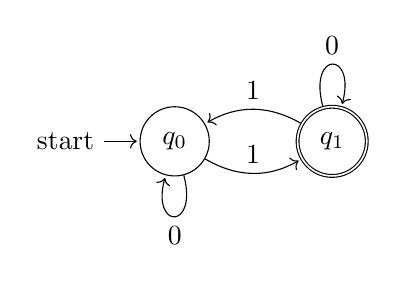
\begin{tikzpicture}[shorten >=1pt, node distance=2cm, on grid, auto]
\node[state, initial] (q_0) {$q_0$};
\node[state, accepting] (q_1) [right=of q_0] {$q_1$};
\path[->]
(q_0) edge [loop below] node {0} ()
	edge [bend right] node {1} (q_1)
(q_1) edge [loop above] node {0} ()
	edge [bend right] node [swap] {1} (q_0);
\end{tikzpicture}.\] Then $L(M)$ consists of all binary strings with an even number of $0$'s.

\item Let $M$ denote
\[
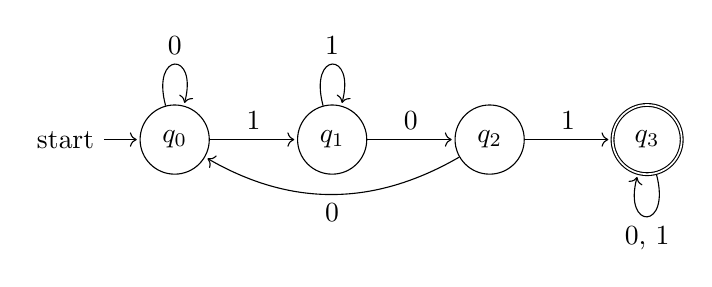
\begin{tikzpicture}[shorten >=1pt, node distance=2cm, on grid, auto]
\node[state, initial] (q_0) {$q_0$};
\node[state] (q_1) [right=of q_0] {$q_1$};
\node[state] (q_2) [right=of q_1] {$q_2$};
\node[state, accepting] (q_3) [right=of q_2] {$q_3$};
\path[->]
(q_0) edge [loop above] node {0} ()
	edge node {1} (q_1)
(q_1) edge [loop above] node {1} ()
	edge node {0} (q_2)
(q_2) edge [bend left] node {0} (q_0)
	edge node {1} (q_3)
(q_3) edge [loop below] node {0, 1} ();
\end{tikzpicture}.
\] Then $L(M) = \left\{x\in \Sigma^{\ast} : x = y101z \text{ for some strings } y \text{ and } z\right\}$.
\end{enumerate}
\end{exmp}

\begin{definition}
A language $L$ is \textit{regular} is there is some $\DFA$ $M$ such that $L(M) = L$.
\end{definition}


Every regular expression induces a $\DFA$, and vice versa. Thus, they have equal expressive power. The former gives rules for generating legitimate strings whereas the latter recognizes membership of a language.


\begin{definition}
A \textit{nondeterministic finite automaton $(\NFA)$} is an ordered quintuple $(Q, \Sigma, q_0, \delta, Q_F)$ of the sort \eqref{eqn:auto} except that $\delta : Q\times \Sigma \to \P(Q)$.
\end{definition}

\begin{exmp} Set $\Sigma = \left\{0,1\right\}$ and $M =$
\[
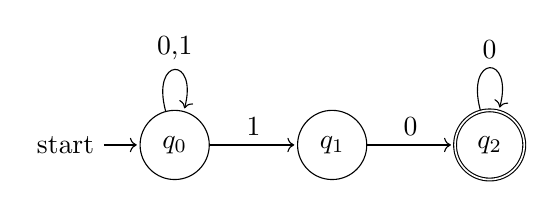
\begin{tikzpicture}[shorten >=1pt, node distance=2cm, on grid, auto]
\node[state, initial] (q_0) {$q_0$};
\node[state] (q_1) [right=of q_0] {$q_1$};
\node[state, accepting] (q_2) [right=of q_1] {$q_2$};
\path[->]
(q_0) edge [loop above] node {0,1} ()
	edge node {1} (q_1)
(q_1) edge node {0} (q_2)
(q_2) edge [loop above] node {0} ();
\end{tikzpicture}.
\] If $x= 0100$, then
\begin{align*} 
& q_0(x) = \{q_0\}
\\ & q_1(x) = \{q_0\}
\\ & q_2(x) = \{q_0, q_1\}
\\ & q_3(x) = \{q_0, q_2\}
\\ & q_4(x) = \{q_0, q_2\}.
\end{align*}
\end{exmp}

\subsection{Lecture 2}


Let $\delta$ denote a transition function for the $\NFA$ $N$. Define the \textit{multi-step transition function} $$\hat{\delta} : Q\times \Sigma^{\ast} \to \P(Q)$$ inductively as follows.
\begin{align*}
 \hat{\delta}(q, \epsilon) & = \{q\}
\\  \hat{\delta} (q, x) & = \bigcup_{\gamma \in \hat{\delta}(q, y)}\delta(\gamma, \sigma) \quad \quad x = y\sigma, \ y \in \Sigma^{\ast}, \ \sigma \in \Sigma.
\end{align*}


Note that if $p\in \hat{\delta}(q,y)$ and $r\in \hat{\delta}(p, \sigma)$, then $r\in \hat{\delta}(q, y\sigma) = \hat{\delta}(q, x)$.


\begin{definition}
A string $x$ is \textit{accepted by $N$} if $\hat{\delta}(q_0, x) \cap Q_F \ne \emptyset$
\end{definition}

\begin{notation}
$L(N) \coloneqq \left\{x \in \Sigma^{\ast} : N \text{ accepts } x\right\}$.
\end{notation}

\smallskip

Every $\DFA$ is an $\NFA$, in which case we have that $\hat{\delta}(q,x) =\left\{\delta\left(\hat{\delta}(q,y), \sigma\right)\right\}$. It's not the case, however, that any $\NFA$ is a $\DFA$.

\smallskip

\begin{theorem}\label{same}
For any $\NFA$ $N$, there is some $\DFA$ $M$ such that $L(N) = L(M)$.
\end{theorem}
\begin{proof}
Let $N = \left(Q, \Sigma, q_0, \delta_N, Q_F\right)$. Define the $\DFA$ $$M \coloneqq \left(\P(Q), \Sigma, q_0^{(1)} , \delta_M, Q_F^{(1)} \right)$$ where $q_0^{(1)} \equiv \{q_0\}$, $\delta_M (Q', \sigma) \equiv \bigcup_{\gamma \in Q'} \delta_N(\gamma, \sigma)$ and $Q_F^{(1)} \equiv \left\{R \subset Q : R\cap Q_F \ne \emptyset\right\}$. For any string $x$, one can use induction on $\left\lvert{x}\right\rvert$ to show that if $R\subset Q$, then $$\tilde{\delta}_M(R, x) = \bigcup_{p\in R} \hat{\delta}_N(p,x)$$ where $\tilde{\delta}_M : \P(Q) \times \Sigma^{\ast} \to \P(Q)$ denotes the obvious extension of $\delta_M$ to strings.  By setting $R= \{q_0\}$, we are done.
\end{proof}

\begin{exmp}
Let $L\subset \{0, 1\}^{\ast}$ consist of those strings $x$ such that $``1010"$ appears in $x$. We can easily capture $L$ with the following $\NFA$, but writing a $\DFA$ that captures $L$ is much harder. 
\[
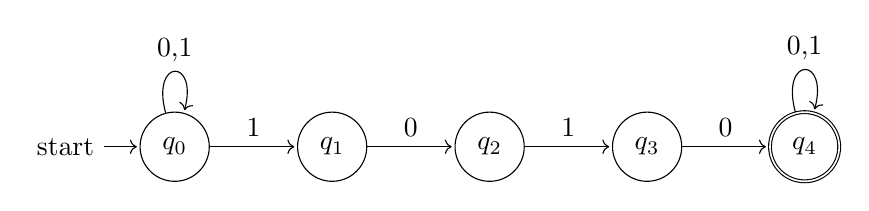
\begin{tikzpicture}[shorten >=1pt, node distance=2cm, on grid, auto]
\node[state, initial] (q_0) {$q_0$};
\node[state] (q_1) [right=of q_0] {$q_1$};
\node[state] (q_2) [right=of q_1] {$q_2$};
\node[state] (q_3) [right=of q_2] {$q_3$};
\node[state, accepting] (q_4) [right=of q_3] {$q_4$};
\path[->]
(q_0) edge [loop above] node {0,1} ()
	edge node {1} (q_1)
(q_1) edge node {0} (q_2)
(q_2) edge node {1} (q_3)
(q_3) edge node {0} (q_4)
(q_4) edge [loop above] node {0,1} ();
\end{tikzpicture}.
\] 
\end{exmp}

\begin{definition} $ $
\begin{enumerate}
\item An $\NFA$ is called an \textit{$\epsilon{-}\NFA$} if its transition function is of the form $\delta: Q\times (\Sigma \cup \{\epsilon\}) \to \P(Q)$. In this case, we call $\delta$ an \textit{$\epsilon$-transition}.
\item  Let $q$ be a state. The \textit{$\epsilon$-closure of $q$} is the set of states that can be reached from $q$ by taking finitely many $\epsilon$-transitions. 
\end{enumerate}
\end{definition}

This determines a function $\epsilon{-}\cl(-): \P(Q) \to \P(Q)$.

\smallskip

\begin{note}
We have that $\hat{\delta}(q, x) = \begin{cases} \epsilon \text{-}\cl(q) & x = \epsilon
\\ \bigcup_{r\in \hat{\delta}(q, y)} \epsilon \text{-}\cl(\delta(r, \sigma)) & x = y\sigma 
\end{cases}.$
\end{note}

\begin{theorem}
For any $\epsilon{-}\NFA$ $N$, there is some $\DFA$ $M$ such that $L(N) = L(M)$.
\end{theorem}
\begin{proof}
Use a similar argument to the proof of \cref{same}. In particular, set $$q_0^{(1)} = \epsilon \text{-}\cl(q_0)$$ and 
\begin{align*}
\delta_M(R, \sigma)  & =  \bigcup_{r\in R}\bigcup_{p\in \epsilon \text{-}\cl(r)} \bigcup_{s\in \delta_N(p, \sigma)} \epsilon \text{-}\cl(s)
\\ & = \bigcup_{r\in R} \bigcup_{s\in \delta_N(r, \sigma)} \epsilon \text{-}\cl(s)
.\end{align*}
\end{proof}

\subsection{Lecture 3}

\begin{prop} Let $L_1, L_2\subset \Sigma^{\ast}$ be regular. 
\begin{enumerate}[label=(\alph*)]
\item $\overline{L_1}\coloneqq \Sigma^{\ast} \setminus L_1 = \left(L_1\right)^c$ is regular.
\begin{corollary}
If $L$ is finite or cofinite, then it is regular.
\end{corollary}
\item $L_1 \cup L_2$ is regular.
\item $L_1 \cap L_2$ is regular. 
\item The language $L_1\cdot L_2 \equiv  \left\{xy \mid x\in L_1 \land y\in L_2\right\}$ is regular. 
\end{enumerate}
\end{prop} 
\begin{proof} By assumption, there exist $\DFA$'s $M_1$ and $M_2$ such that $L_1 = L(M_1)$ and $L_2 = L(M_2)$.
\begin{enumerate}[label=(\alph*)]
\item Construct a new $\DFA$ $M_3$ by making every final state of $M_1$ non-final and vice versa. Then $L(M_3) = \overline{L_1}$.
\item Construct an $\epsilon{-}\NFA$ $M_3$ as follows. Take a starting state $q_0$. Attach  an $\epsilon$-transition  from $q_0$ to the starting state of $M_1$  and  an $\epsilon$-transition from $q_0$ to the starting state of $M_2$. Then $L(M_3) = L_1 \cup L_2$.
\item Note that $L_1 \cap L_2 = \left(\overline{L_1} \cup \overline{L_2}\right)^c$.  Now apply (a) and (b).
\item Construct an $\epsilon{-}\NFA$ $M_3$ as follows. Given any final state $q$ of $M_1$, add an $\epsilon$-transition from $q$ to the start state of $M_2$. Then $L(M_3) = L_1\cdot L_2$.
\end{enumerate}
\end{proof}

\medskip

Now, let $L$ be any language. Let $L^k \coloneqq \underbrace{L\cdot L \cdots L}_{k \text{ times}}$ for each integer $k\geq 1$. Moreover, let $L^0 = \{\epsilon\}$ (which is regular). Then let $$L^{\ast} = \bigcup_{k\geq 0} L^k.$$

\medskip

\begin{prop}
If $L$ is regular, then $L^{\ast}$ is regular as well.
\end{prop}
\begin{proof}
There is some $\DFA$ $M$ such that $L(M) =L$. Without loss of generality, write $M$ as
\[
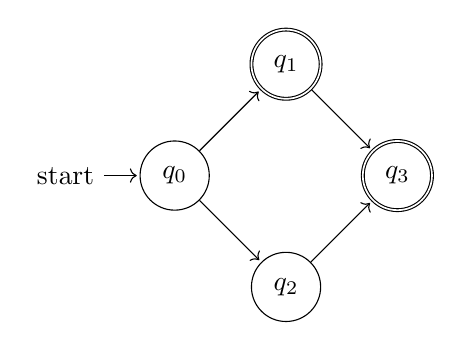
\begin{tikzpicture}[shorten >=1pt,node distance=2cm,on grid,auto] 
   \node[state,initial] (q_0)   {$q_0$}; 
   \node[state, accepting] (q_1) [above right=of q_0] {$q_1$}; 
   \node[state] (q_2) [below right=of q_0] {$q_2$}; 
   \node[state,accepting](q_3) [below right=of q_1] {$q_3$};
    \path[->] 
    (q_0) edge  node {} (q_1)
          edge  node [swap] {} (q_2)
    (q_1) edge  node { } (q_3)
    (q_2) edge  node [swap] {} (q_3);
\end{tikzpicture}.
\] Now, let $\widetilde{M}$ denote the automaton
\[
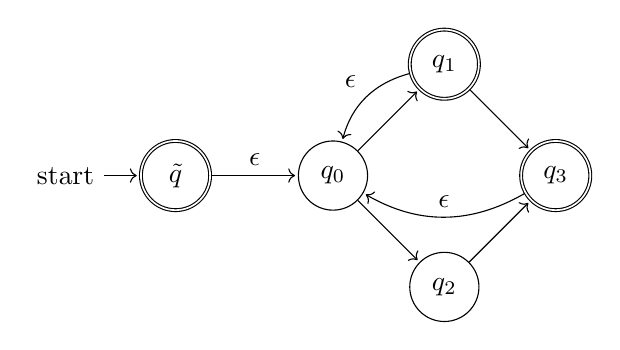
\begin{tikzpicture}[shorten >=1pt,node distance=2cm,on grid,auto] 
   \node[state,initial, accepting] (q)   {$\tilde{q}$}; 
      \node[state] (q_0) [right=of q] {$q_0$};
   \node[state, accepting] (q_1) [above right=of q_0] {$q_1$}; 
   \node[state] (q_2) [below right=of q_0] {$q_2$}; 
   \node[state,accepting](q_3) [below right=of q_1] {$q_3$};
    \path[->]
      (q) edge  node {$\epsilon$} (q_0)
    (q_0) edge  node {} (q_1)
          edge  node [swap] {} (q_2)
    (q_1) edge  node { } (q_3)
    	edge  [bend right] node [swap] {$\epsilon$} (q_0)
    (q_2) edge  node [swap] {} (q_3)
    (q_3) edge [bend left] node [swap] {$\epsilon$} (q_0);
\end{tikzpicture}.
.\] Then $L\left(\widetilde{M}\right) = L^{\ast}$.
\end{proof}

\smallskip

There exists a canonical set isomorphism $\left\{F: F \text{ is a finite automaton}\right\} \cong \N$. Also, we have that $\left\{0,1\right\}^{\ast} \cong \N$. But then $\R \cong \P(\N) \cong \P(\left\{0,1\right\}^{\ast}) = \left\{L : L \text{ is a language over } \left\{0,1\right\}\right\}$. Since there is a surjection $$\left\{F: F \text{ is a finite automaton}\right\} \to \left\{L : L \text{ is a regular language over } \left\{0,1\right\}\right\},$$ it follows that there are uncountably many non-regular languages over $\left\{0,1\right\}$.


\subsection{Lecture 4}

\begin{lemma}[Pumping] Let $L$ be a regular language. Then there exists $n_0 \in \N$ such that for any $x\in L$ with $\left\lvert{x}\right\rvert\geq n_0$, we may write $x=wyz$ such that
\begin{enumerate}[label=(\alph*)]
\item $\left\lvert{y}\right\rvert >0$,
\item $\left\lvert{wy}\right\rvert\leq n_0$, and
\item if $i\geq 0$, then $wy^iz \in L$ where $y^i \coloneqq \underbrace{y\cdots y}_{i \text{ times}}$.
\end{enumerate}
In this case, we call the minimal such $n_0$ the \textit{pumping length of $L$}.
\end{lemma}
\begin{proof}
By assumption, there is some $\DFA$ $M = (Q, \Sigma, \delta, q_0, Q_F)$ such that $L = L(M)$. Let $n_0 = \left\lvert{Q}\right\rvert$. Let $x\in L$ such that $\left\lvert{x}\right\rvert\geq n_0$. Set $q_i = \hat{\delta}(q_0, x_0 \cdots x_i)$ for each $i\geq 0$.  There exist $0\leq i<j \leq n_0$ such that $q_i = q_j$. Consider the three strings 
\begin{gather*}
w\coloneqq x_1\cdots x_i 
\\  y\coloneqq  x_{i+1}\cdots x_j 
\\  z\coloneqq x_{j+1} \cdots x_m.
\end{gather*}
where $\left\lvert{x}\right\rvert = m$. It is straightforward to verify that these satisfy conditions (a), (b), and (c).
\end{proof}
\begin{corollary} $ $
\begin{enumerate} 
\item Our last proof shows that any regular language $L$ has pumping length $\leq \left\lvert{Q}\right\rvert$.
\item If $L(M) \ne \emptyset$, then there exists $x\in L(M)$ such that $\left\lvert{x}\right\rvert \leq \left\lvert{Q}\right\rvert$.
\end{enumerate}
\end{corollary}

\begin{exmp} Let $n_0\geq 0$ be an integer. Suppose that $x=wyz$ with $\left\lvert{y}\right\rvert >0$ and $\left\lvert{wy}\right\rvert\leq n_0$.
\begin{enumerate}
\item Let $L=  \left\{ 1^{2^n} : n\geq 0\right\}$. Let $x= 1^{2^{n_0+1}}$.  Note that $$\left\lvert{wy^iz}\right\rvert = \left\lvert{wyz}\right\rvert + (i-1)\left\lvert{y}\right\rvert = 2^{n_0+1} + (i-1)\left\lvert{y}\right\rvert.$$ Hence if $i=2$, then $\left\lvert{wy^i z}\right\rvert = 2^{n_0+1} +\left\lvert{y}\right\rvert \leq 2^{n_0+1} +n_0 < 2^{n_0+2}$ since $n_0 < 2^{n_0+1}$, in which case $2^{n_0+1} < \left\lvert{wy^i z}\right\rvert$ as well. Therefore, $L$ is not a regular language. 
\item Let $L = \left\{ ww : w \in \left\{0,1\right\}^{\ast}\right\}$. Let $x= 0^{n_0}10^{n_0}1$. If $\left\lvert{y}\right\rvert= m$ with $0<m\leq n_0$,  then $wz= 0^{n_0-m}10^{n_0}1$, which does not belong to $L$. Hence $L$ is \emph{not} a regular language. 
\end{enumerate}
\end{exmp}

\begin{aside}
Let $D$ be a $\DFA$ with $\left\lvert{Q_D}\right\rvert =n$. Then $D$ recognizes an infinite language if and only if it accepts some string $s$ such that $n\leq \left\lvert{s}\right\rvert \leq 2n$.
\end{aside}
\begin{proof}
The ($\Longleftarrow$) direction follows from the pumping lemma. Conversely, suppose that $L(D)$ belongs tofinite. Then $D$ contains some path $p$ of states from the start state to a final state as well as some cycle of states $c$ such that $c \cap p \ne \emptyset$. Note that $\left\lvert{c}\right\rvert \leq n$ and $\left\lvert{p}\right\rvert \leq n$. Hence we can apply $c$ sufficiently many times to get our desired string.
\end{proof}

\section{Computability theory}

\begin{definition}[Turing machine]
A \textit{Turing machine} is a $7$-tuple $$\left(Q, \Sigma, \Gamma, \delta, q_0, Q_F, Q_R\right)$$ where $\Gamma \supset \Sigma$ is finite such that 
\begin{enumerate}[label=(\roman*)]
\item there is some \textit{null character} $\bot \in \Gamma \setminus \Sigma$,
\item $\delta : Q\times \Gamma \to Q \times \Gamma \times \{L, R\}$, 
\item and $Q_F, Q_R \subset Q$ such that $Q_F \cap Q_R = \emptyset$. 
\end{enumerate}
We call $\Sigma$ the \textit{input alphabet}, $\Gamma$ the \textit{tape alphabet}, $Q_F$ the set of \textit{accepting states}, and $Q_R$ the set of \textit{rejecting states}.
\end{definition}

\begin{note}
On any given input $x$, a $\TM$ can either \textit{accept} or \textit{reject} or \textit{loop} (i.e., fail to halt on $x$).
\end{note}

\smallskip

A Turing machine is supposed to act as a minimal model of computation. It should be able to write, be able to move left and right, and have unconstrained memory.


\subsection{Lecture 5}


Every finite automaton may be viewed as a Turing machine $M$ with the following properties. 
\begin{enumerate}[label=(\alph*)]
\item $M$ never writes on the tape.
\item $M$'s read-write head moves to the right only.
\item $M$ writes on just a finite portion of the tape.
\item $M$ either accepts or rejects immediately after reading the input string. 
\end{enumerate}


\begin{remark}
Adding a stay option $S$ to the set $\{L, R\}$ would not increase a Turing machine's computational power.
\end{remark}

\begin{definition}
Let $M$ be a Turing machine. Let $q\in Q$ and $u,v\in \Gamma^{\ast}$. We say that the \textit{configuration of $M$} is $uqv$ if 
\begin{enumerate}[label=(\alph*)]
\item the current state of $M$ is $q$,
\item the current tape contents is precisely $uv$, and
\item the current head location is the first symbol of $v$.
\end{enumerate}
We call this an \textit{accepting configuration} if $q \in Q_F$ and a \textit{rejecting configuration} if $q \in Q_R$.
\end{definition}

\begin{definition}
Let $a,b,c\in \Gamma$ and $u,v\in \Gamma^{\ast}$. Let $p,q\in Q$. We say that the configuration $C_1$ \textit{yields} the configuration $C_2$ in the following cases:
\begin{enumerate}[label=(\alph*)]
\item $uapbv$ yields $uqacv$ when $\delta(p,b) = (q, c, L)$.
\item $uapbv$ yields $uacqv$ when $\delta(p, b) = (q, c, R)$. 
\end{enumerate}
In this case, we write $C_1 \vdash C_2$.
\end{definition}

\medskip

We say that the $\TM$ $M$ \textit{accepts} the input $w$ if 
\begin{enumerate}[label=(\roman*)]
\item there is some sequence $C_1, \ldots, C_k$ of configurations such that $C_1$ is $\bot q_0w$, 
\item each $C_i$ yields $C_{i+1}$ (in which case we write $C_1 \specialvdash{}{*} C_k $), 
\item and $C_k$ is an accepting configuration. 
\end{enumerate}
We define the \textit{language of the $\TM$ $M$} as $$L(M) \equiv \left\{x \in \Sigma^{\ast}: M \text{ accepts } x \right\}.$$

\smallskip

\begin{definition} Let $L$ be a language.
\begin{enumerate}
\item We say that $L$ is \textit{Turing-recognizable} or \textit{recursively enumerable} if there is some $\TM$ $M$ such that $L = L(M)$.
\item We say that $L$ is \textit{decidable} or \textit{recursive} if there is some $\TM$ $M$ such that $L= L(M)$ and $M$ halts on every input. In this case, we say that $M$ is an \textit{algorithm}.
\end{enumerate}
\end{definition}

\begin{note}
Every decidable language is recursively enumerable. 
\end{note}

\begin{exmp}
By the pumping lemma, one may show that the language $L\coloneqq \left\{0^n1^n : n\geq 1\right\}$ is \emph{not} regular.  But $L$ is decidable. Indeed,
set $\Sigma = \left\{0,1\right\}$ and $\Gamma = \Sigma \cup \{\bot, +, \times\}$. Define the $\TM$ $M$ as follows.
\[
\begin{tikzpicture}[shorten >=1pt,node distance=6cm,on grid,auto] 
   \node[state,initial] (q_0)   {$q_0$}; 
   \node[state, accepting] (q_1) [right=of q_0] {$q_1$}; 
    \node[state](q_2) [right=of q_1] {$q_2$};
   \node[state] (q_3) [below=of q_0] {$q_3$}; 
    \node[state,accepting] (q_4) [right=of q_3] {$q_4$};
    \path[->] 
    (q_0) edge  node {0/$+$, R} (q_1)
          edge  node[swap] {$\times$/$\times$, R} (q_3)
    (q_1) edge  node {1/$\times$, L } (q_2)
    		edge [loop below] node { $\times$/$\times$, R} ()
		edge [loop above] node {0/0, R } ()
    (q_2) edge [bend left]  node {$+$/$+$, R} (q_0)
    	edge [loop below] node {$\times$/$\times$, L } ()
		edge [loop above] node {0/0, L } ()
    (q_3) edge  node {$\bot$/$\bot$, R } (q_4)
    	edge [loop left] node {$\times$/$\times$, R } ()
    ;
\end{tikzpicture}.
\]
Then $L(M) = L$.
\end{exmp}

\begin{remark}
The \textit{Church-Turing thesis} states that our pre-theoretic notion of algorithm is entirely captured by decidability (equivalently, $\lambda$-computability). 
\end{remark}

\subsection{Lecture 6}

\begin{definition}
A \textit{multi-tape Turing machine} is exactly like an ordinary Turing machine except that the former's transition function is of the form $$ \delta : Q \times \Gamma^k \to Q \times \Gamma^k \times \{L, R\}^k  $$ where $k\in \N$.
\end{definition}

\begin{theorem}\label{equiv}
For any $k\in \N$ and any language $L$, if there is some $k$-tape $\TM$ $M$ such that $L(M) = M$, then there is some single-tape $\TM$ $M'$ such that $L = L(M')$. Moreover, $T$ steps of a $k$-tape $\TM$ can be simulated using $O_k(T^2)$ steps of a single-tape $\TM$.
\end{theorem}
\begin{proof}
Write $M= \left(Q, \Sigma, \Gamma, \delta, q_0, Q_F, Q_R\right)$. Let $$ \{\#\} \bigcup_{\gamma \in \Gamma} \{\gamma, \dot{\gamma} \}$$ be the tape alphabet of $M'$. Construct $M'$ so that its tape always has $\#$ in a cell separating  the current contents of $M$'s different tapes and $\dot{\gamma}$ whenever the head of the tape of $M$ containing $\gamma$ is currently at $\gamma$. We make $M'$ scan its tape once to determine the positions of the heads of $M$'s tapes, then scan it again to update its contents according to $\delta$.
\end{proof}

\begin{exmp}
Let $L = \left\{w \in \left\{0,1\right\}^{\ast} \mid w \text{ is a palindrome}\right\}$. This cannot be recognized by a $\TM$ running in better than quadratic time  but can be recognized by a $2$-tape $\TM$ running in linear time.  Thus, computational models may differ in complexity even when they don't in decidability.
\end{exmp}

\begin{definition}
A \textit{nondeterministic Turing machine} $M$ is exactly like an ordinary Turing machine except that $M$'s transition function is of the form $$ \delta : Q \times \Gamma \to \P(Q \times \Gamma \times \{L, R\})  $$ such that $M$ accepts on an input as long as at least one branch of computation accepts.
\end{definition}

\begin{theorem}\label{LT}
Let $M$ be a $\NDTM$ and let $L = L(M)$. Then there exists a $\TM$ $M'$ such that $L= L(M')$. 
\end{theorem}
\begin{proof}
By \cref{equiv}, it suffices to construct a multi-tape $\TM$ that simulates $M$. Construct a tree with branches corresponding to threads of computation given by $M$ and nodes corresponding to configurations of $M$. We construct a $3$-tape $\TM$ $D$ as follows. 

\medskip

 Tape 1 always contains the input string $w$ and nothing else. Tape 2 contains just the string on the tape of the current node. Setting $m = \max\{ \left\lvert{A}\right\rvert : A \in \im{\delta} \}$, tape 3 contains a string over $\{1, \ldots, m\}$ that corresponds to the ``address" of the current node. 

\medskip

 We make $D$ simulate a breadth-first search of the tree as follows. 
\begin{enumerate}
\item Initialize  tape 1 with $w$ and tape $3$ with $\epsilon$. 
\item Copy tape 1 to tape 2.
\item Move to the node given by the next symbol on tape 3.
\item Read the configuration of $M$ on $w$ that is determined by this node.
\item Accept or reject if this is an accepting or rejecting configuration, respectively. 
\item Replace the current string on tape 3 with the next string under the string order.
\item Do step 1.
\end{enumerate}
\end{proof}

\begin{note} $ $
\begin{enumerate}
\item This simulation has time complexity $O(m^T)$ where $T$ denotes the steps taken by $M$.
\item We can modify the proof of \cref{LT} to show that if $M$ always halts on each branch of computation, then $M'$ always halts. Thus, a language is decidable if and only if a $\NDTM$ decides it.
\end{enumerate}
\end{note}

\medskip

There is an injective function $\iota$ from the set of Turning machines into $\left\{0,1\right\}^{\ast}$ because any $\TM$'s transition function admits a finite description. In particular, the set of $\TM$ is countable. Let $\langle M \rangle $ denote the binary encoding of the $\TM$ $M$. Let any $x\notin \im{\iota}$ correspond to the $\TM$ that immediately halts and outputs zero on every input. As a result, every binary string corresponds to some Turing machine. 

\smallskip

\begin{theorem}
 There is a $\TM$ (denoted by $U_{\TM}$) taking two strings as inputs, $\langle M \rangle$ and $x$, (i.e., one string over $\left\{0,1\right\} \times \Sigma$) such that
 \begin{enumerate}[label=(\alph*)]
 \item if $M$ accepts $x$, then $U_{\TM}$ accepts,
 \item if $M$ rejects $x$, then $U_{\TM}$ rejects, and
 \item if $M$ does not halt on $x$, then neither does $U_{\TM}$.
 \end{enumerate} Moreover, if $M$ takes $T$ steps on $w$, then $U_{\TM}$ takes $O(T \log{T})$ steps on $\langle M, w \rangle$.
\end{theorem}
\begin{proof}
This is like constructing an interpreter for a programming language within the language itself. See Theorem 1.13 (Arora and Barak) for a high-level proof.
\end{proof}

\begin{term}
We call $U_{\TM}$ a \textit{universal Turing machine}.
\end{term}

\subsection{Lecture 7}


Alternatively, we can view $U_{\TM}$ as a ternary function with input $\left(\langle M \rangle,  w, 1^k\right)$ such that
\begin{enumerate}[label=(\roman*)]
\item if $M$ accepts (resp. rejects) on $w$ in $\leq k$ steps, then $U_{\TM}$ accepts (resp. rejects) and
\item if $M$ does not halt on $w$ in $\leq k$ steps, then $U_{\TM}$ will reach a special state.
\end{enumerate}


\begin{lemma}
Let $A_{\TM}$ denote the language $\{ \langle M, w \rangle \mid M$ accepts $w\}$. Then $A_{\TM}$ is recursively enumerable.
\end{lemma}
\begin{proof}
Simply observe that $L(U_{\TM}) = A_{\TM}$.
\end{proof}

\begin{theorem}
$A_{\TM}$ is undecidable.
\end{theorem}
\begin{proof}
Suppose, toward a contradiction, that there is some $M$ that decides $A_{\TM}$.  Design a new $\TM$ $N$ as follows.
\begin{enumerate}[label=(\alph*)]
\item Given a binary string $x$, run $M$ on $(\langle M_x \rangle, \langle M_x \rangle)$ where $M_x$ denotes the $\TM$ corresponding to $x$.
\item Let $N$ reject when $M$ accepts and $N$ accept when $M$ rejects.
\end{enumerate}

Then $$N(\langle N \rangle) = \begin{cases} \textit{accept} & N \text{ does not accept } \langle N \rangle \\ \textit{reject} & N \text{ accepts } \langle N \rangle    \end{cases},$$ which is impossible. 
\end{proof}

\begin{lemma}
If $L$ is decidable, then  $\overline{L}$ is decidable.
\end{lemma}

\begin{lemma}
If both $L$ and $\overline{L}$ are recursively enumerable, then $L$ is decidable. 
\end{lemma}
\begin{proof}
Find some $M_1$ and $M_2$ such that $L = L(M_1)$ and $\overline{L} = L(M_2)$. Construct some $\TM$ $M$ as follows. 

\smallskip

\begin{algorithm}[H]
    \SetKwInOut{Input}{Input}
    \Input{the string $w$}
    {$T=1$}\;
    \While{the current state is a non-halting state}
      {
        run $U_{\TM}$ on $(\langle M_1 \rangle, w) $ for $T$ steps\;
        \eIf{$U_{\TM}$ accepts}{accept}{run $U_{\TM}$ on $(\langle M_2 \rangle, w)$ for $T$ steps \;
        \eIf{$U_{\TM}$ accepts}{reject}{$T$\texttt{ += }1}
      }  }
      \caption{pseudocode describing $M$}
\end{algorithm}

\end{proof}

\begin{corollary}
$\overline{A_{\TM}}$ is not recursively enumerable. 
\end{corollary}

\begin{definition}
A function $f: \Sigma^{\ast} \to \underline{\Sigma}^{\ast}$ is \textit{computable} if there is some $\TM$ $M$ such that for any string $w$, $M$ halts on $w$ with its tape containing just $f(w)$. 
\end{definition}

\begin{definition}
Let $L\subset \Sigma^{\ast}$ and $L' \subset \underline{\Sigma}^{\ast}$ be languages. We say that \textit{$L$ many-one reduces to $L'$}, written as $L \leq_m L'$, if there is some computable function $f: \Sigma^{\ast} \to \underline{\Sigma}^{\ast}$ such that $$x\in L \iff f(x) \in L'.$$ In this case, we call $f$ the \textit{reduction} from $L$ to $L'$.
\end{definition}

\begin{lemma}
Suppose that $L \leq_m L'$ and that $L'$ is decidable (resp. recursively enumerable), then $L$ is decidable (resp. recursively enumerable).
\end{lemma}
\begin{proof}
Find some $M$ that decides (resp. recognizes) $L'$ and some reduction $f$ from $L$ to $L'$. Construct the $\TM$ $N$ so that on input $w\in \Sigma^{\ast}$, we let $N$ compute $f(w)$ and then output whatever $M$ outputs on $f(w)$. Then $N$ decides (resp. recognizes) $L$. 
\end{proof}

In this way, $L'$ is at least as ``hard" as $L$.

\subsection{Lecture 8}

\begin{exmp}[Halting problem]
Let $A_{\text{HALT}} = \{\langle M, w \rangle \mid M$ halts on $w\}$. Then $A_{\text{HALT}}$ is undecidable.
\end{exmp}
\begin{proof}
Recall that $A_{\TM}$ is undecidable. Thus, it suffices to show that $A_{\TM} \leq_m A_{\text{HALT}}$. To do this, we want to design a computable function that maps any $\langle M, w \rangle$ to another $\langle M' \rangle, w'$ such that $M'$ halts on $w'$ precisely when $M$ accepts $w$. Construct such an $M'$ as follows.

\smallskip

\begin{algorithm}[H]
    \SetKwInOut{Input}{Input}
    \Input{the string $x$}
    {run $U_{\TM}$ on $(\langle M \rangle, x)$}\;
     \eIf{$U_{\TM}$ accepts}{accept}{
     \While{true}{pass}
     } 
      \caption{pseudocode describing $M'$}
\end{algorithm}

\smallskip

Then we get a suitable function given by $(\langle M \rangle , w) \mapsto (\langle M' \rangle, w)$.
\end{proof}


\begin{theorem}[Rice]
 Let $C$ be any subset of the universe of all languages over a fixed alphabet. Let $$L_C = \left\{ \langle M \rangle : L(M) \in C\right\}.$$ Suppose that both $L_C$ and $\overline{L_C}$ are nonempty. Then $L_C$ is undecidable. 
\end{theorem}
\begin{proof}
We may assume that $\emptyset \notin C$ for otherwise we could show that $\overline{L_C}$ is undecidable.  We know that $L(M_y) \in C$ for some $\TM$ $M_y$.  We show that $A_{\TM} \leq_m L_C$. Consider any $\langle M, w \rangle \in A_{\TM}$. Define $M'$ as follows.

\smallskip

\begin{algorithm}[H]
    \SetKwInOut{Input}{Input}
    \Input{the string $x$}
    {run $U_{\TM}$ on $\langle M, w \rangle$}\;
     \eIf{$U_{\TM}$ accepts}{run $U_{\TM}$ on $\langle M_y, x \rangle$}{
    reject
     } 
      \caption{pseudocode describing $M'$}
\end{algorithm}

\smallskip

If $M$ accepts $w$, then $L(M') = L(M_y)$. If $M$ rejects $w$, then $L(M') = \emptyset$. If $M$ does not halt on $w$, then $L(M') = \emptyset$.
\end{proof}

\smallskip

This means that every nontrivial semantic property of Turing machines is undecidable.

\medskip

\begin{exmp}\label{fin}
Let $A_{\fin} = \left\{\langle M \rangle : L(M) \text{ is finite}\right\}$. Then $A_{\fin}$ is undecidable. 
\end{exmp}

\smallskip

In fact, we can strengthen \cref{fin}.

\smallskip

\begin{prop}
$A_{\fin}$ is not recursively enumerable. 
\end{prop}
\begin{proof}
Recall that $\overline{A_{\TM}}$ is not recursively enumerable.  We show that $\overline{A_{\TM}} \leq_m A_{\fin}$. Given any $\langle M, w \rangle$, define $M'$ as follows.

\smallskip

\begin{algorithm}[H]
    \SetKwInOut{Input}{Input}
    \Input{the string $x$}
    {run $U_{\TM}$ on $\langle M, w \rangle$}\;
     \eIf{$U_{\TM}$ accepts}{accept}{
    reject
     } 
      \caption{pseudocode describing $M'$}
\end{algorithm}

\smallskip

If $M$ accepts $w$, then $L(M') = \left\{0,1\right\}^{\ast}$. Otherwise, $L(M') = \emptyset$.  
\end{proof}

\begin{note}
It's possible that both a language and its complement are not recursively enumerable. 
\end{note}

\section{Complexity theory}

\subsection{Lecture 9}


Once we know that a question is decidable, we want to determine the amount of computational resources required to decide it. Such resources include 
\begin{itemize}
\item time
\item space
\item parallelism 
\item communication 
\item rounds
\item randomness
.\end{itemize}
We also want to study how these trade off with each other. 

\smallskip

\begin{definition}[Time complexity]
Given any $\TM$ $M$, its \textit{time complexity} is the function $f: \N \to \N$ where $$f(n) \equiv\max\{\text{steps used by }M \text{ on input }w\mid \left\lvert{w}\right\rvert =n\}.$$ We say that $M$ \textit{runs in time $f(n)$}.
\end{definition}

\smallskip

 Given any \textit{time-constructible} function $f: \N \to \N$, let $$\mathsf{DTIME}(f(n)) = \left\{ L : \exists \TM \ M  \text{ s.t. } L = L(M) \text{ and }M \text{ halts on all inputs of length }n \text{ in }O(f(n)) \text{ steps}\right\}.$$
Let $\mathbf{P} = \bigcup_{k\geq 0} \mathsf{DTIME}(n^k)$.


\begin{prop}
$\mathbf{P}$ belongs todependent of the variant of deterministic Turing machine used. 
\end{prop}

\begin{remark}
Given any convex body, we want to compute its volume. In 1989, Dyer and Frieze proved that this is solvable in $O(n^{23})$ steps. It is now known that it's solvable in $O(n^2)$ steps. 
\end{remark}

\begin{exmp}
For any $k\geq 0$, $\mathsf{DTIME}(n^k) \subset \mathsf{DTIME}(n^{k+1})$. Consider the case where $k=2$. Then we can show that this containment  is proper by using diagonalization. Indeed, define the language $L$ as follows. 
\begin{enumerate}
\item If $x$ is of the form $w10^i$ for some $w$ and some $i$, then let $x\notin L$.
\item Otherwise, let $M_w$ be the $\TM$ corresponding to $w$. 
\item In this case, run $M_w$ on $x$ for $n^2$ steps where $n$ denotes $\left\lvert{x}\right\rvert$. 
\item  If $M_w$ does not halt in so many steps, then let $x\notin L$. 
\item Else, let $x\in L$ when $M_w$ rejects and let $x\notin L$ when $M_w$ accepts. 
\end{enumerate}
Steps 2 and 3 together take $O(n^2 \log{n})$ steps. It follows that $L \in \mathsf{DTIME}(n^2\log{n})\subset \mathsf{DTIME}(n^3)$. But $L \notin \mathsf{DTIME}(n^2)$.
\end{exmp}

\begin{theorem}[Time hierarchy]
Let $f: \N \to \N$ be any function. Suppose that $g(n) = \omega(f(n) \log{f(n)})$. Then $\mathsf{DTIME}(f(n)) \subsetneq \mathsf{DTIME}(g(n))$.
\end{theorem}

\begin{definition}
We say that a $\NDTM$ $M$ has \textit{time complexity} $t(n)$ if every branch of $M$ runs in time $t(n)$. 
\end{definition}

\smallskip

Let  $$\mathsf{NTIME}(t(n)) = \left\{ L : \exists \NDTM M \text{ s.t. }L(M) = L \text{ and every branch of }M\text{ halts on any input of length }n\text{ in }O(t(n))\text{ steps}\right\}.$$ Let $\mathbf{NP} = \bigcup_{k \geq 0} \mathsf{NTIME}(n^k)$.

\begin{prop}
$\mathsf{NTIME}(t(n)) \subset \mathsf{DTIME}(2^{O(t(n))})$.
\end{prop}

\begin{exmp}
Let $\varphi$ be a Boolean formula in conjunctive normal form (CNF). Suppose that $\varphi$ contains $n$ clauses and $m$ literals. Then the size of the representation in bits of $\varphi$ is of order $O(2 m \cdot n) = O(mn)$. Also, deciding whether $\varphi$ evaluates to $1$ takes  $O(2 m \cdot n) = O(mn)$ steps. 

Let $\mathsf{CNF\text{-}SAT} = \left\{\langle \varphi \rangle : \varphi \text{ is satisfiable}\right\}$. Notice that this can be decided by a nondeterministic Turing machine in linear time.  There is, however, no known deterministic Turing machine running faster than brute force. 
\end{exmp}

\subsection{Lecture 10}

\begin{lemma}
A language $L$  belongs to $\NP$ if and only if there exist  a deterministic $\TM$ $V(\cdot, \cdot)$ and constants $c_1, c_2 >0$ such that $$L = \left\{ x \mid \exists y.\left\lvert{y}\right\rvert \leq \left\lvert{x}\right\rvert^{c_1} \land V(x,y) = 1 \text{ where } V \text{ runs in time }\left\lvert{x\cdot y}\right\rvert^{c_2}\right\}.$$ In this case, we call $V$ a \textit{verifier} and $y$ a \textit{witness}.
\end{lemma}
\begin{proof} $ $

($\Longrightarrow$) 

\smallskip

There is some $\NDTM$ $M$ running in polynomial time such that $L(M) = L$. Say that $M$ runs in time $n^c$. The sequence of choices along any branch of $M$ can be represented by a binary string of length $n^c$.
Define $V$ as the algorithm taking inputs $x$ and $y$ with $y\in  \left\{0,1\right\}^{n^c}$ and executing $M$ on $x$ with choice of branch given by $y$. Then $V$ runs in polynomial time, and $x\in L \iff V(x,y) =1$ for some $y$.

\medskip


($\Longleftarrow$)  

\smallskip

Given an input $x$, define a $\NDTM$ $M$ that first guesses a witness $y$ in a separate tape and then runs $V$ on $(x,y)$ in polynomial time. 
\end{proof}

\begin{note}
Equivalently, we could have made $V$ run in time $\left\lvert{x}\right\rvert^{c_2}$ while dropping the requirement that $\left\lvert{y}\right\rvert$ be polynomial in $\left\lvert{x}\right\rvert$. 
\end{note}

\begin{definition}
An \textit{independent set} of a graph $G=\left(V, E\right)$ is a set $I\subset V$ such that no two points in $I$ are connected by an edge. 
\end{definition}

\begin{exmp} The following languages are in $\NP$.
\begin{enumerate}
\item $\mathsf{IND{-}SET} \coloneqq \{\langle G, k \rangle : G$ is an (undirected) graph with an independent set of size at least $k\}$
\item $\mathsf{3{-}COLOR}\coloneqq \left\{ \langle G \rangle : G\text{ has a }3\text{-coloring}\right\}$.
\item $\mathsf{Composite} \coloneqq \left\{x \mid x\text{ is a composite number}\right\}$.
\item $\mathsf{PRIMES}\coloneqq \left\{ n \mid n\text{ is prime}\right\}$.
\end{enumerate}
\end{exmp}

\begin{definition}
We say that $L_1$ \textit{polynomially many-one reduces to} $L_2$ (written as $L_1 \leq_m^p L_2$) if there is some $\TM$ $M$ running in polynomial time such that $x \in L_1 \iff M(x) \in L_2$.
\end{definition}

\begin{lemma}
If $L_1 \leq_m^p L_2$ and $L_2 \in \mathbf{P}$, then $L_1 \in \mathbf{P}$.
\end{lemma}

\begin{definition}
We say that $L$ is $\NP$-complete if $L \in \NP$ and for any $L' \in \NP$, $L' \leq_m^p L$. 
\end{definition}

\subsection{Lecture 11}

\begin{definition}
A \textit{(Boolean) circuit} is a directed acyclic graph with a unique sink node such that 
\begin{enumerate}[label=(\roman*)]
\item each node has indegree at most $2$,
\item each internal node is labelled by $ \land$, $\vee$, or $\neg$,
\item each leaf  node is labeled by a Boolean variable, and
\item each edge is labeled by the Boolean value given as the output of the prior node. 
\end{enumerate}
The \textit{size of a circuit} is the number of its internal nodes.
\end{definition}

\begin{remark}
This is an example of a non-uniform model of computation as we must specify a new circuit for each input size. 
\end{remark}

\begin{lemma}\label{pl1}
Every function $g: \left\{0,1\right\}^n \to \left\{0,1\right\}$ can be computed by a circuit of size $O(2^n)$. 
\end{lemma}
\begin{proof}
We use induction to show that any function $g:\left\{0,1\right\}^n \to \left\{0,1\right\}$ can be computed by a circuit of size at most $3 \cdot 2^n -4$, which is enough. When $n=1$, there are four cases to consider.
\begin{enumerate}[label=(\alph*)]
\item If $g= \id_{\left\{0,1\right\}}$, then $g$ can be computed by a circuit of size $0$.
\item If $g(0) =1$ and $g(1) =0$, then $g(x) = \neg{x}$.
\item If $g(0) = g(1) = 0$, then $g(x) = x \land \neg{x}$.
\item If $g(0) = g(1) = 1$, then $g(x) = x \vee \neg{x}$.
\end{enumerate}
Hence the base case holds. Now, define $g_0, g_1 : \{0,1 \}^{n-1} \to \left\{0,1\right\}$ by $g_0(y) = g(0, y)$ and $g_1(y) = g(1,y)$. Then $g$ satisfies $$g(y) = (\neg y_1 \land g_0(y_2, \ldots, y_n)) \vee (y_1 \land g_1(y_2, \ldots, y_n))$$ for each $y$. By induction, $g$ can be computed by a circuit of size at most $4 + 2(3 \cdot 2^{n-1} -4) = 3 \cdot 2^n -4$. 
\end{proof}

\begin{lemma}\label{pl2}
Let $M= \left(Q, \Sigma, \Gamma, q_0, \delta, Q_F, Q_R\right)$ be a $\TM$. Suppose that on any input of size $n$, $M$ halts in at most $t$ steps with $t\geq n$. Then there is a circuit of size $O(t^2 \cdot (\left\lvert{\Gamma}\right\rvert\cdot \left\lvert{Q}\right\rvert)^3) = O(t^2)$ that  outputs $1$ on a  string $x$ of length $n$ if and only if $M$ accepts $x$.
\end{lemma}
\begin{proof}
We want to encode a given configuration of $M$, which we may assume uses at most $t$ cells of tape. To do this, we take $\log{\left\lvert{\Gamma}\right\rvert}$ bits, $1$ bit, and $\log{\left\lvert{Q}\right\rvert}$ bits to encode the content of the current cell, whether or not the head is located at this cell, and, if so, the current state, respectively.  For each $i,j\geq0$, the bit $b_{j, l+1}$ representing the $j$-th cell at time $l+1$ depends precisely on the three bits $b_{j-1, l}$, $b_{j, l}$, and $b_{j+1, l}$. If $B\coloneqq 1+ \log{\left\lvert{\Gamma}\right\rvert} +\log{\left\lvert{Q}\right\rvert}$, then every bit of the encoding of the configuration of $M$ at time $l+1$ depends on $3B$ bits. This determines a Boolean function $f: \left\{0,1\right\}^{3B}\to \left\{0,1\right\}$ that computes the next configuration. \Cref{pl1} implies that $f$ be be computed by a circuit of size $O(2^{3B})$ and hence by one of size $O(\left(\left\lvert{\Gamma}\right\rvert\cdot \left\lvert{Q}\right\rvert\right)^3)$. Thus, there is a circuit of size $O(t\cdot t\cdot  \left(\left\lvert{\Gamma}\right\rvert \cdot \left\lvert{Q}\right\rvert\right)^3 )$ that simulates $M$ on inputs of size $n$.
\end{proof}

\begin{exmp}[Cook-Levin theorem]
Let  $\mathsf{CIRCUIT{-}SAT} = \left\{ \langle C \rangle : \exists x. C(x) = 1\right\}$. This is certainly in $\NP$. We claim that it is $\NP$-complete.
\end{exmp}
\begin{proof}
If $L \in \NP$, then there is an efficient (i.e.,  polynomial-time) algorithm $V$ such that $$\forall x\in L.\exists y\in \Sigma^{\ast}.\left\lvert{y}\right\rvert\leq \left\lvert{x}\right\rvert^{O(1)} \land V(x,y) =1 \land (x\notin L \implies \forall y. V(x,y)=0).$$ Thus, for each $n\in \N$, we can use \cref{pl2} to construct a circuit of size $n^{O(1)}$ such that $C(x,y) = V(x,y)$ for each string $x$ of size $n$ and each string $y$ with $\left\lvert{y}\right\rvert\leq n^{O(1)}$. This means that for each string $x$, we can construct a circuit $C_x(\cdot)$ of size $\left\lvert{x}\right\rvert^{O(1)}$ such that $C_x(y) = V(x,y)$ for any $y$ with $\left\lvert{y}\right\rvert\leq \left\lvert{x}\right\rvert^{O(1)}$. The mapping $M: x\mapsto \langle C_x(\cdot) \rangle$ satisfies $x\in L \iff M(x) \in \mathsf{CIRCUIT{-}SAT}$, as desired.  
\end{proof}

\subsection{Lecture 12}

\begin{corollary}\label{cc1}
Showing that $\mathsf{CIRCUIT{-}SAT}$ is not in $\mathbf{P}$ is equivalent to showing that $\mathbf{P} \ne \NP$.
\end{corollary}

\begin{corollary}\label{cc2}
Suppose that $\mathsf{CIRCUIT{-}SAT} \leq_m^p L$ and $L\in \NP$. Then any $L' \in \NP$ satisfies $L' \leq_m^p L$, i.e., $L$ is $\NP$-complete.
\end{corollary}

\smallskip

\Cref{cc1} and \cref{cc2} hold with $\mathsf{CIRCUIT{-}SAT}$ replaced by any $\NP$-complete language. 

\smallskip

\begin{definition}
A Boolean formula in CNF is a \textit{3cnf formula} if each clause contains exactly $3$ literals.  
\end{definition}

\begin{exmp} $ $
\begin{enumerate}
\item Consider $\mathsf{3{-}SAT}\coloneqq \left\{\langle \varphi \rangle \mid \varphi\text{ is a 3cnf formula that is satisfiable}\right\}$. This is certainly in $\NP$. We claim that it is $\NP$-complete.
\begin{proof}
It suffices to show that $\mathsf{CIRCUIT{-}SAT} \leq_m^p \mathsf{3{-}SAT}$. We must construct an efficient algorithm $M( -)$ such that the circuit $C$ is satisfiable  if and only if $\varphi\coloneqq M(\langle C \rangle)$ is satisfiable. If $C$ has size $n$, then, wlog, we can use the associativity of our Boolean operations to add at most $n^k$ internal nodes to $C$ such that each gate labeled by $\land$ or $\vee$ takes exactly two inputs. 

Let $g_1, \ldots, g_n$ and $x_1, \ldots, x_m$ denote  the Boolean values given by the edges and inputs of $C$, respectively. Relabel $g_1, \ldots, g_n, x_1, \ldots, x_m$ as $w_1, \ldots, w_{n+m}$. Let $\varphi$ be the 3cnf formula in the variables $w_1, \ldots, w_{n+m}$ where each clause of $\varphi$ corresponds either to $C$'s output value $w_s \vee w_s \vee w_s$ or to one of $C$'s internal edges. In the latter case, we can give the following descriptions.
\begin{itemize}
\item  If $w_j = \neg w_i$, then $\varphi$ contains exactly one clause of the form $$  \left(w_i \vee w_j\right) \land \left(\neg w_i \vee \neg w_j\right).
$$
\item If $w_h = w_i \land w_j$ in $C$, then $\varphi$ contains exactly one clause of the form $$  \left(w_i \vee w_j \vee \neg w_h\right) \land \left(w_i \vee \neg w_j \vee \neg w_h\right) \land \left(\neg w_i \vee w_j \vee \neg w_h\right) \land \left(\neg w_i \vee \neg w_j \vee w_h\right).$$
\item If $w_h = w_i \vee w_j$ in $C$, then $\varphi$ contains exactly one clause of the form $$ \left(w_i \vee w_j \vee \neg w_h\right) \land \left(w_i \vee \neg w_j \vee w_h\right) \land \left(\neg w_i \vee w_j \vee w_h\right) \land \left(\neg w_i \vee \neg w_j \vee w_h\right)
.$$
\end{itemize} By construction, $\varphi$ is satisfiable if and only if $C$ is. The algorithm $M: \langle C \rangle \mapsto \varphi$ is linear in $n^k$, hence efficient. Therefore, it is a suitable reduction. 
\end{proof}
\item  It's clear that $\mathsf{IND{-}SET}$ belongs to $\NP$. We claim that this is $\NP$-complete.
\begin{proof}
We show that $\mathsf{3{-}SAT} \leq_m^p \mathsf{IND{-}SET}$.  Let $\varphi$ be a 3cnf-formula and let $$\varphi = c_1 \land c_2 \land c_3 \land \cdots \land c_m.$$ For each clause $c_i$, create a triangle $t_i$ with vertices corresponding to the three literals in $c_i$. Let $G_{\varphi}$ denote the graph obtained from the graph $\coprod_{i=1}^m t_i$ by adding an edge between any two conflicting vertices $v$ and $\neg v$ in $\coprod_{i=1}^m t_i$. Then the algorithm $\varphi \mapsto \langle G_{\varphi}, m\rangle$ defines a suitable reduction. 
\end{proof}
\item We say that $K \subset V$ is a \textit{vertex cover} of a graph $G=\left(V, E\right)$ if any $(x,y) \in E$ has $x\in K$ or $y\in K$. Define $\mathsf{VC}= \left\{ \langle G, k\rangle \mid G\text{ has a vertex cover of size at most }k\right\}$. Then $\mathsf{IND{-}SET} \leq_m^p \mathsf{VC}$, so that $\mathsf{VC}$ is $\NP$-complete.  
\begin{proof}
Let $G$ be a graph with an independent set $S$ with $\left\lvert{S}\right\rvert\geq k$.  Then $V \setminus S$ is a vertex cover of $G$. Conversely, if $G$ has a vertex cover $K$ of size at most $\left\lvert{V}\right\rvert - k$, then $V \setminus K$ is an independent set of size at least $k$ in $G$. Thus, the algorithm $\langle G, k \rangle \mapsto \langle G, \left\lvert{V}\right\rvert - k\rangle$ defines a suitable reduction.  
\end{proof}
\end{enumerate}
\end{exmp}

\subsection{Lecture 13}

\begin{definition}
We say that a language $L$ is \textit{$\NP$-hard} if $L' \leq_m^p L$ for any $L' \in \NP$.
\end{definition}

\begin{definition} Let $G=\left(V, E\right)$ be a graph
\begin{enumerate}
\item A subset $C \subset V$ is a \textit{clique in $G$} if any two distinct points in $C$ are adjacent. Let $$\mathsf{CLIQUE}= \left\{\langle G, k \rangle \mid G \text{ has a clique of size at least }k\right\}.$$
\item The graph $\overline{G} = (V, E')$ where $E' \equiv \left\{(x,y) \mid (x,y) \notin E\right\}$ is the  \textit{complement graph of $G$}.
\end{enumerate}
\end{definition}

\begin{prop}
 A set $S$ of vertices in a graph $G$ is an independent set in $G$ if and only if it is a clique in $\overline{G}$.
\end{prop}

\begin{exmp}
$\mathsf{IND{-}SET} \leq_m^p \mathsf{CLIQUE}$ via the mapping $\langle G, k \rangle \mapsto \langle \overline{G}, k \rangle$. Hence $\mathsf{CLIQUE}$ is $\NP$-hard.
\end{exmp}

\begin{definition}
Let $G= \left(V, E\right)$ be an (undirected) weighted graph with weight function $w : E \to \R_{\geq 0}$. Suppose that $C \subset V$. A \textit{Steiner tree in $G$} is a connected subgraph of $G$ with no cycles that contains each vertex in $C$.
\end{definition}

\begin{remark}
Any connected subgraph of minimum weight must be a tree.
\end{remark}

\medskip

\begin{prob}
Given a weighted graph $G$ and set of vertices $C$ in $G$, find the Steiner tree in $G$ of minimum weight that contains $C$.
\end{prob}

\begin{definition}
Let $G= \left(V, E\right)$. A subset $C\subset V$ \textit{has a Steiner tree of total weight $W$} if there exists a connected subgraph of $G$ that contains every vertex in $C$ and has weight at most $W$.
\end{definition}

\begin{exmp}
Let $\mathsf{Steiner{-}tree} = \left\{\langle G, C, W \rangle \mid C\text{ has a Steiner tree of total weight at most }W\right\}$. This is $\NP$-complete.
\end{exmp}
\begin{proof}
It's clear that $\mathsf{Steiner{-}tree} $ belongs to  $\NP$. To show that it is also $\NP$-hard, we prove that $\mathsf{VC} \leq_m^p \mathsf{Steiner{-}tree} $. Let $G = \left(V, E\right)$ be a graph with a vertex cover $S$ of size $k$. 
 Let $$V' = \bigcup_{v \in V} [v] \bigcup_{(u,v) \in E}[u,v].$$ Build $E'$ as follows. 
\begin{enumerate}[label=(\alph*)]
\item Let $([u], [v])\in E'$ for any $u,v \in V$ and set $w'([u], [v])=1$. 
\item If $(u,v) \in E$, then let $\left([u], [u,v]\right), \left([u, v], [v]\right) \in E'$ and set $w'([u], [u,v]) = w'([u,v], [v]) =1$. 
\item If $(v,w) \in E$ and $u,v,w$ are pairwise distinct, then let $\left([u], [v,w]\right) \in E'$ and and set $w'([u], [v,w]) = 2$.
\item Finally, for any $(u,v), (w,z) \in E$, let $\left([u,v], [w,z]\right)\in E'$  with weight $$w'([u,v], [w,z])\equiv \begin{cases} 2 & (u,v) \text{ and } (w,z) \text{ share a vertex} \\ 3 & \text{otherwise} \end{cases}.$$ 
\end{enumerate}
Set $C = \left\{ [u,v] : (u,v) \in E\right\}$. Also, set $W= \left\lvert{E}\right\rvert+ k -1$. Let $G' = \left(V', E', w'\right)$. Note that we have constructed $G'$ in polynomial time.
\begin{claim}
$G'$ has a Steiner tree containing $C$ with weight at most $\left\lvert{E}\right\rvert + k -1$.
\end{claim}
\begin{proof}
Let $S = \{v_1, \ldots, v_k\}$. Let 
\begin{align*}
S' & = \left\{[v_1], \ldots, [v_k], \ \bigcup_{(u,v) \in E}[u,v]\right\}
\\ E_{S'} & = \left\{ (x,y)\in E' \mid w'(x,y)=1 \text{ and } x,y\in S'\right\}.
\end{align*} Since $S$ is a vertex cover, we see that $(S', E_{S'})$ is a connected subgraph of $G'$ that contains $C$ and has weight $\left\lvert{E}\right\rvert+k -1$.
\end{proof}
\begin{claim}
If $C$ has a a Steiner tree $T$ of total weight $W \leq \left\lvert{E}\right\rvert +k -1$, then $G$ has a vertex cover of size $k$. 
\end{claim}
\begin{proof}
Alter $T$ as follows.
\begin{itemize}
\item Replace any edge of weight $2$ between $[w]$ and $[u,v]$ with the edges $\left([w], [u]\right)$ and $\left([u], [u,v]\right)$.
\item Replace any edge of weight $2$ between $[u,v]$ and $[v,w]$ with the edges $\left([u,v], [v]\right)$ and $\left([v], [v,w]\right)$.
\item Replace any edge of weight $3$ between $[u,v]$ and $[w,z]$ with the edges $\left([u,v], [v]\right)$, $\left([v], [w]\right)$, and $\left([w], [w,z]\right)$.
\end{itemize}
The resultant graph $T'$ is connected and contains $C$. Note that $T'$ has weight at most $\left\lvert{E}\right\rvert + k -1$ where each edge of $T'$ has weight $1$. This implies that $T'$ spans at most $\left\lvert{E}\right\rvert +k$ vertices. Since $T'$ contains $C$, it follows that $T'$ contains a set $R$ of vertices of the form $[v]$ such that $\left\lvert{R}\right\rvert\leq k$. If $(x,y)\in E$, then $[x,y]$ is connected to some $[v_0]$ by edges of weight $1$. This means that $[x]$ or $[y]$ belongs to $T'$, so that $[x]$ or $[y]$ belongs to $R$. This shows that $R$ is a vertex cover for $G$.
\end{proof}
\end{proof}

\begin{remark}
Any undirected  weighted (connected) graph can be endowed with a metric by taking the shortest path between any two vertices. Our choice of weights in part (d) of our construction of $E'$ makes $G'$ a metric space. 
\end{remark}

\begin{exmp}
Let $\mathsf{SUBSET{-}SUM} = \left\{\langle a_1, \ldots, a_k, t\rangle \mid a_i,t\geq 0,\ \exists S \subset [k].\sum_{i\in S} a_i = t\right\}$. Then $\mathsf{SUBSET{-}SUM}$ is $\NP$-complete.
\end{exmp}
\begin{proof}
It's clear that this belongs to $\NP$. We show that $\mathsf{VC} \leq_m^p \mathsf{SUBSET{-}SUM}$. Let $G=\left(V, E\right)$ such that $\left\lvert{V}\right\rvert = n$ and $\left\lvert{E}\right\rvert= m$. We can make $E$ totally ordered. Suppose that $G$ has a vertex cover $C$ of size $k$. For each $v\in V$, we define an integer $a_v\geq 0$ in base-4 (written from left to right) consisting of $m+1$ digits. Further, for each $e\in E$, we define an integer $b_e\geq 0$ in base-4 consisting of $m+1$ digits. Specifically, if $0\leq i \leq \left\lvert{E}\right\rvert-1$ and  $(u,v) \in E$ is the $i$-th edge, then define both $a_u$ and $a_v$  as the integer $$0 \cdots 0 \underbrace{1}_{i\text{-th digit}} 0 \cdots 01   $$ and define $b_{(u,v)}$ as the integer $$0 \cdots 0 \underbrace{1}_{i\text{-th digit}} 0 \cdots 00     .$$ Now, set $t= k \cdot 4^m + \sum_{i=0}^{m-1}2 \cdot 4^i$.

\medskip

 Let $S = \left\{a_v \mid v\in C\right\} \cup \left\{b_{(u,v)} \mid\text{ exactly one of }u\text{ and }v\text{ belongs to }C\right\}$. Note that we can construct $S$ in polynomial time. It's straightforward to check that the terms of $S$ sum to $t$. 
\begin{claim}
Suppose that there are subsets $U\subset V$ and $T\subset E$ such that $$t= \sum_{u\in U}a_u +\sum_{(u,v) \in T} b_{(u,v)}.$$ Then $U$ is a vertex cover for $G$ of size at most $k$.
\end{claim}
\begin{proof}
Since $t<(k+1)4^m$ and each $a_u> 4^m$, it follows that $\left\lvert{U}\right\rvert\leq k$. Note that, in base-4, each of the first $m$ digits of $t$ equals $2$. Thus, for each $(u,v) \in E$, at least two of $a_u$, $a_v$, and $b_{(u,v)}$ contribute to the summation $$\sum_{u\in U}a_u +\sum_{(u,v) \in T} b_{(u,v)}.$$ This implies that at least one of $u$ and $v$ belongs to $U$. Hence $U$ is a vertex cover for $G$.
\end{proof}
\end{proof}

\begin{remark}
Using dynamic programming, one can show that there is a poly$(k, t)$ algorithm deciding $\mathsf{SUBSET{-}SUM}$. This result, however, does not imply that $\mathsf{SUBSET{-}SUM} \in \mathbf{P}$, because the size of the whole input $\langle a_1, \ldots, a_k, t\rangle$ is on the order of \hl{$k\log{t}$}.
\end{remark}

\subsection{Lecture 14}

Let $S: \N \to \N$. Unless we state otherwise, we assume that $S(n) \geq \log{n}$.
Consider the \textit{space complexity class} 
$\mathsf{DSPACE}(S(n))$ consisting of all languages $L$ for which $$\exists \TM M\text{ s.t. }L = L(M) \text{ and on any input of length }n,\ M \text{ touches at most }S(n)\text{ cells (on its work tape)}.$$
Further, let $\mathsf{NSPACE}(S(n))$ consist of all languages $L$ for which  there is some $\NDTM M\text{ s.t. } L = L(M)$ and
\[
\text{on any input of length }n,\ M\text{ halts on every branch of computation and touches at most }S(n)\text{ cells on any branch}.
\]


\begin{definition}
Let $M$ be a Turing machine that always halts. Define the \textit{configuration graph $G_{M,x}$ of $M$ on input $x$} as the directed graph $\left(V, E\right)$ where $V$ consists of the possible configurations of $M$ on $x$ and $E \equiv \left\{(C,C') : C \vdash C'\right\}$.
\end{definition}

 By making $M$ erase the contents of its work tapes right before halting, we may assume that $M$ has exactly one accepting configuration $C_{\accpt}$ on $x$.
Moreover,
since $M$ always halts, it can never reach the same configuration more than once. Thus, $G_{M,x}$ is a directed acyclic graph.  


\begin{lemma}
$\mathsf{NSPACE}(S(n)) \subset \mathsf{DTIME}(2^{O(S(n))})$.
\end{lemma}
\begin{proof}
Let $L \in \mathsf{NSPACE}(S(n)) $ with $L(M) = L$.  Given any input $x$ of length $n$, we can use $O(S(n))$ bits to describe the current contents of the tape, $O(\log{S(n)})$ bits to describe the current state, and $O(1)$ bits to describe the current location of the head. Thus, we need $$O(S(n)) + O(1) + O(\log{S(n)})= O(S(n))$$ bits to describe any vertex of $G_{M,x}$. 

\medskip


Note that the number of configurations of $M$ is at most $2^{O(S(n))}$ (provided that any configuration of a $\NDTM$ yields at most two distinct configurations).  Therefore, we can construct $G_{M,x}$ in $2^{O(S(n))}$ steps. Now apply the standard linear-time breadth-first search for connectivity to $G_{M,x}$ to decide if there is a path from $C_{\mathrm{start}}$ to $C_{\accpt}$. 
\end{proof}


\begin{corollary} $ $
\begin{enumerate}
\item $\mathsf{DTIME}(S(n)) \subset \mathsf{DSPACE}(S(n)) \subset \mathsf{NSPACE}(S(n)) \subset \mathsf{DTIME}(2^{O(S(n))})$.
\item $\mathsf{DTIME}(S(n)) \subset \mathsf{NTIME}(S(n)) \subset \mathsf{NSPACE}(S(n))$.
\end{enumerate}
\end{corollary}

\begin{remark}
It is not known whether these chains of containment can be improved. 
\end{remark}

\begin{notation} $ $
\begin{enumerate}
\item $\mathsf{PSPACE} \coloneqq \bigcup_{k\geq 0} \mathsf{DSPACE}(n^k)$.
\item $\mathsf{NPSPACE} \coloneqq \bigcup_{k \geq 0} \mathsf{NSPACE}(n^k)$.
\end{enumerate}
\end{notation}

\begin{note} $ $
\begin{enumerate}
\item $\mathbf{P} \subset \mathsf{PSPACE}$.
\item $\NP \subset \mathsf{NPSPACE}$.
\end{enumerate}
\end{note}

\begin{prop}
Let $\mathbf{L} = \mathsf{DSPACE}(\log{n})$ and $\mathbf{NL}= \mathsf{NSPACE}(\log{n})$. 
\begin{enumerate}
\item Let $L_1 = \left\{\langle x,y,z \rangle \mid x \cdot y = z\right\}$ and $L_2 = \left\{\langle x,y,z \rangle \mid x+y = z\right\}$. Then $L_1, L_2 \in \mathbf{L}$.
\item Let $\mathsf{DIR{-}REACH} = \left\{\langle G, s, t \rangle \mid G\text{ is directed and the vertex }t\text{ is reachable from }s\right\}$. Then $\mathsf{DIR{-}REACH}  \in \mathbf{NL}$.
\begin{remark}
Omer Reingold has shown that $$\mathsf{REACH} \coloneqq  \left\{\langle G, s, t \rangle \mid G\text{ is undirected and the vertex }t\text{ is reachable from }s\right\}$$ belongs to $\mathbf{L}$.
\end{remark}
\end{enumerate}
\end{prop}

\smallskip

Recall that $\mathsf{NTIME}(S(n)) \subset \mathsf{DTIME}(2^{O(S(n))})$. The corresponding relation for space complexity, however, is much better

\begin{theorem}[Savitch]
 $\mathsf{NSPACE}(S(n)) \subset \mathsf{DSPACE}(S^2(n))$.
\end{theorem}

\begin{corollary}
$\mathsf{PSPACE} = \mathsf{NPSPACE}$.
\end{corollary}

\subsection{Lecture 15}

\begin{theorem}[Savitch]\label{Sav}
 $\mathsf{NSPACE}(S(n)) \subset \mathsf{DSPACE}(S^2(n)).$
\end{theorem}
\begin{proof}
Let $L \in \mathsf{NSPACE}(S(n)) $ with $L(M) = L$. Recall that the configuration graph $G_{M,x}$ has at most $T_0\coloneqq 2^{O(S(n))}$ nodes. Consider the following recursive algorithm.

\smallskip

\begin{algorithm}[H]
    \SetKwInOut{Input}{Input}
    \Input{the string $x$}
    \For{$j \in \{1, \ldots, T_0\}$}
   {\eIf{$\mathsf{REACH}(C_{\mathrm{start}}, j, \frac{T_0}{2})$ and $\mathsf{REACH}( j, C_{\accpt}, \frac{T_0}{2})$}{output ``yes"}{output ``no"}}
\end{algorithm}


Denote the space complexity of the preceding algorithm by $\mathcal{L}(T_0)$. Note that we we can reuse the space used by the first recursive call for the second recursive call. Since we need $\log{T_0}$ cells to encode the counter, it follows that
$$  \mathcal{L}(T_0) = \log{T_0} + \mathcal{L}(T_0/2) + O(1) .   $$   Note that the recursion depth here is precisely $\log{T_0}$. Using this, we compute
\begin{align*}  \mathcal{L}(T_0)  & =    \log{T_0} + \mathcal{L}(T_0/2) 
\\ & = \log^2{T_0} + \mathcal{L}(1) =  \log^2{2^{O(S(n))}} + \mathcal{L}(1) 
\\ & = O(S^2(n)) + O(S(n)) = O(S^2(n))  .
\end{align*}
\end{proof}

\begin{corollary}
$\mathbf{NL} \subset \mathbf{P}$.
\end{corollary}
\begin{proof}
The follows because $\mathsf{DIR{-}REACH}$ is  $\mathbf{NL}$-complete and, by our proof of \cref{Sav}, has a $\log^2{n}$-space deterministic algorithm.
\end{proof}

\begin{note} $ $
\begin{enumerate}
\item $\mathsf{NTIME}(\text{poly}(n)) \subset \mathsf{NPSACE}(\text{poly}(n)) \subset \mathsf{DPSACE}(\text{poly}(n)) = \mathsf{PSPACE}.$
\item $\mathsf{PSPACE}$ is closed under complementation. 
\end{enumerate}
\end{note}

\begin{exmp} $ $
\begin{enumerate}
\item Let $\Sigma_2{-}\mathsf{SAT} = \left\{\varphi \text{ Boolean} \mid \forall \bar{x} \exists \bar{y}(\varphi(\bar{x}, \bar{y}) = 1)\right\}$. It is unclear that this (or its complement) belongs to $\NP$. 
\item Let $\mathsf{TQBF{-}SAT} = \left\{ \varphi(\overline{x_1}, \ldots, \overline{x_n}) \mid Q_1 \overline{x_1} Q_2 \overline{x_2}Q_3 \overline{x_3} \cdots Q_n \overline{x_n} (\varphi(\overline{x_1}, \ldots, \overline{x_n}) = 1), \ Q_i \in \{\forall, \exists\} \right\}$. This stands for the set of \textit{totally quantified Boolean formulas}. It belongs to $\mathsf{PSPACE}$.
\begin{proof}
Construct an algorithm $T(\varphi)$ as follows. 
\begin{itemize}
\item If $\varphi$ is quantifier-free, then evaluate it directly. Accept if it evaluates to $1$ and reject otherwise. 
\item If $\varphi = \exists x \psi$, then recursively call $T$ on $\psi$ once with $x=0$ and once with $x=1$. Accept if either of these recursive calls accepts and reject otherwise. 
\item If  $\varphi = \forall x \psi$, then recursively call $T$ on $\psi$ once with $x=0$ and once with $x=1$. Accept if both of these recursive calls accept and reject otherwise. 
\end{itemize} 
If $m$ denotes the size of $\varphi$, then $$\mathcal{L}(m) = m^{O(1)} + \mathcal{L}(m-1) + O(1) = m^{O(1)} + \mathcal{L}(m-1) = O(m^k)$$ for some $k$.
\end{proof}
\end{enumerate}
\end{exmp}

\subsection{Lecture 16}

\begin{definition}
A language $L$ is $\mathsf{PSPACE}$-complete if it belongs to $\mathsf{PSPACE}$ and for any $L' \in \mathsf{PSPACE}$, $L' \leq_m^p L$.
\end{definition}

\begin{exmp}
$\mathsf{TQBF{-}SAT} $ is $\mathsf{PSPACE}$-complete.
\end{exmp}
\begin{proof}
Let $L \in \mathsf{PSPACE}$ with $L(M) = L$. Given any input $x$ with $\left\lvert{x}\right\rvert =n$, we want to construct a TQBF $\varphi_{c, c', i}$ of size $O(S(n)^2)$ that is is satisfiable if and only if there is a path of length at most $2^i$ from $c$ to $c'$ in the configuration graph $G_{M,x}$. This will imply that $$\hat{\varphi}\coloneqq \varphi_{C_{\mathrm{start}}, C_{\accpt}, O(S(n))}$$ is true if and only if $M$ accepts $x$ if and only if $x\in L$.


 We have previously constructed such a $\varphi_{c_1, c_2, 0}$. Moreover, if $i\geq 1$, then we see that 
\begin{align*}
\varphi_{c_1, c_2, i} & \leftrightarrow \exists c(\varphi_{c_1, c, i-1} \land \varphi_{c, c_2, i-1})
\\ & \leftrightarrow \exists c \forall D^1 \forall D^2((D^1 = c_1 \land D^2 = c) \vee (D^1 = c) \land (D^2 = c_2)) \implies \varphi_{D^1, D^2, i-1}.
\end{align*}
It follows that $\left\lvert{\varphi_{c_1, c_2, i}}\right\rvert\leq \left\lvert{\varphi_{c_1, c_2, i-1}}\right\rvert +O(S(n))$, so that $\left\lvert{\hat{\varphi}}\right\rvert \leq O(S(n)^2)$, as desired.
\end{proof}

\begin{prop}
A language $L$ belongs to $\mathbf{NL}$ if and only if there exist $c\in \N$ and a deterministic $\TM$ $V(\cdot, \cdot)$ consisting of one read-only input tape, one work tape, and one read-only, single-axis proof tape  such that $V$'s work tape uses $O(\log{\left\lvert{\text{(first input)}}\right\rvert})$ space and $$L = \left\{ x \mid \exists y.\left\lvert{y}\right\rvert \leq \left\lvert{x}\right\rvert^{c} \land V(x,y) = 1\right\}.$$ .
\end{prop}

\subsection{Lecture 17}

\begin{definition} $ $
\begin{enumerate}
\item
Let $M$ be a $\TM$ consisting of one read-only input tape, one work tape, and one write-only, single-axis output tape such that $M$'s work tape uses $O(\log{n})$ space. We call $M$ a \textit{log space transducer}.
\item Let $A$ and $B$ be languages. We say that $A$ is \textit{log space reducible to $B$}, written as $A\leq_l B$, if there is some log space transducer $M: \Sigma^{\ast} \to \underline{\Sigma}^{\ast}$ such that $x \in A \iff M(x) \in B$. 
\item A language $L$ is \textit{$\mathbf{NL}$-complete} if it belongs to $\mathbf{NL}$ and $L' \leq_l L$ for any $L' \in \mathbf{NL}$.
\end{enumerate}
\end{definition}

\begin{prop}
If $L \in \mathbf{NL}$ and $L' \leq_l L$, then  $L' \in \mathbf{NL}$.
\end{prop}

\begin{exmp}
$\mathsf{DIR{-}REACH}$ is $\mathbf{NL}$-complete.\footnote{Theorem 4.16 (Arora and Barak).}
\end{exmp}

\begin{theorem}[Immerman-Szelepcs\'enyi]
$$\mathbf{NL} = \mathbf{co}{-}{\mathbf{NL}}.$$
\end{theorem}
\begin{proof}
Since $\mathsf{DIR{-}REACH}$ is $\mathbf{NL}$-complete, it suffices to show that $\mathsf{DIR{-}REACH}^c\in \mathbf{NL}.$  
Let $G= \left(V, E\right)$ be a graph of size $n$ and $s, t\in V$. Let $C_i$ denote the set of vertices $v\in V$ reachable from $s$ in at most $i$ steps. We can assume that $V$ is ordered $\left(v_1, \ldots, v_n\right)$ since each index can be described in $\log{n}$ bits.

\medskip

First, let $v\in V$. Given that $\left\lvert{C_i}\right\rvert = k$, we can verify that $v \notin C_i$ as follows. 
\begin{enumerate}
\item Propose a list $v_{s_1}, \ldots, v_{s_m}$ of vertices and a path $s\leadsto v_{s_i}$ for each $1\leq i \leq m$. 
\item Write the next $v_{s_i}$ on the work tape and write the proposed path $s \leadsto v_{s_i}$ on the proof tape. 
\item Verify that the proposed path is valid. If not, then \textit{reject}.
\item Otherwise, verify that $s_i > s_{i-1}$ and $v_{s_i} \ne v$. If not, then \textit{reject}. 
\item \text{Repeat steps 2-4} until there is no $v_{s_i}$ left. 
\item Verify that $m = k$ by using a counter on the work tape. If not, then \textit{reject}. Otherwise, \textit{accept}.
\end{enumerate}

Second, given that $\left\lvert{C_{i-1}}\right\rvert = k$,  we can verify that $v\notin C_i$ as follows.
\begin{enumerate}
\item Propose a list $v_{s_1}, \ldots, v_{s_m}$ of vertices and a path $s\leadsto v_{s_i}$ for each $1\leq i \leq m$. 
\item Write the next $v_{s_i}$ on the work tape and write the proposed path $s \leadsto v_{s_i}$ on the proof tape. 
\item Verify that the proposed path is valid. If not, then \textit{reject}.
\item Otherwise, verify that $s_i > s_{i-1}$, $v_{s_i} \ne v$, and \underline{$v_{s_i}$ is not a neighbor of $v$}. If not, then \textit{reject}. 
\item \text{Repeat steps 2-4} until there is no $v_{s_i}$ left. 
\item Verify that $m = k$ by using a counter on the work tape. If not, then \textit{reject}. Otherwise, \textit{accept}.
\end{enumerate}

Finally, let $c\in \N$. Given that $\left\lvert{C_{i-1}}\right\rvert=k$, we can verify that $\left\lvert{C_i}\right\rvert = c$ as follows. 
\begin{enumerate} 
\item Write the next $v_i$ on the work tape (where $1\leq i \leq n$). 
\item Decide if $v_i \in C_i$ using our two previous algorithms.
\item Repeat steps 1-2 until there is no $v_i$ left.
\item Determine the number $r$ of vertices in $C_i$ by using a counter on the work tape. If $r = c$, then \textit{accept}. Otherwise, \textit{reject}.
\end{enumerate}

Note that each of our three verifiers uses $O(\log{n})$ space on its work tape and  is polynomial in $n$ on its proof tape. Apply our final algorithm iteratively $n$-times to verify the size of  $C_n$. Since we can reuse space on the work tape, our space complexity on it remains $O(\log{n})$.  Next, apply our first algorithm to verify that $t\notin C_n$, in which case $t$ is not reachable from $s$.
\end{proof}

\begin{corollary}
If $s(n) \geq \log{n}$, then $\mathsf{NSPACE}(s(n)) = \mathbf{co}{-}\mathsf{NSPACE}(s(n))$.
\end{corollary}

\begin{remark}
Thanks to Bertrand's postulate, some prime number between $N$ and $2N$ always exists.  Suppose that we want to find the least such prime $\tilde{p}$. Consider the probability $\mathbb{P}$ that a randomly chosen number between $N$ and $2N$ is prime. From the prime number theorem, it is known that $\mathbb{P} \approx \frac{N}{\log{N}}$. As a result, we can apply the AKS primality test $O(\log{N})$ times to find $\tilde{p}$ with high probability.
\end{remark}

\subsection{Lecture 18}

\begin{definition} $ $
\begin{enumerate}
\item We call a $\TM$ a \textit{probabilistic/randomized Turing machine} if it consists of an input tape, a work tape, and a ``random bits" tape.  
\item Let $p: \N \to \N$ be a polynomial. A probabilistic $\TM$ $M({\cdot}, {\cdot})$ \textit{decides $L$ with respect to $p$} if 
\begin{itemize}
\item for any $x\in L$, $\mathbb{P}_{r\in_R \left\{0,1\right\}^{p(\left\lvert{x}\right\rvert)}}[M(x,r)=1] \geq \frac{2}{3}$ and
\item for any $x\notin L$, $\mathbb{P}_{r\in_R \left\{0,1\right\}^{p(\left\lvert{x}\right\rvert)}}[M(x,r)=0] \geq \frac{2}{3}$.
\end{itemize}
\end{enumerate}
\end{definition}

\begin{definition} $ $
A language $L$ belongs to $$\underbrace{\mathsf{BPTIME}(t(n))}_{\textit{bounded error probabilistic time}}$$ if there exists a randomized $\TM$ $M$ running in time $t(\left\lvert{x}\right\rvert)$ (with probability $1$) such that $M$ decides $L$ with respect to $t(n)$. Let $\mathbf{BPP}= \bigcup_{c\geq 0} \mathsf{BPTIME}(n^c)$.
\end{definition}

\begin{note}
It's clear that $\mathbf{P} \subset \mathbf{BPP}$.
\end{note}

\begin{prop}
$\mathbf{P} \ne \mathbf{NP} \implies \mathbf{P} = \mathbf{BPP}$.
\end{prop}

\bigskip

\begin{remark} $ $
\begin{enumerate}
\item Computing the value of the determinant of an $n\times n$ matrix of integers via cofactor expansion takes $\omega(n!)$ steps. Computing it via Gaussian elimination, however, takes $O(n^3)$ steps. 
\item Computing the value of the determinant of an $n\times n$ matrix of linear forms over $\Z$ via cofactor expansion is exponential in $n$. There is no known deterministic polynomial time algorithm for such a computation.
\end{enumerate}
\end{remark}

\begin{prop}\label{poly} $ $
\begin{enumerate}[label=(\alph*)]
\item Let $L$ be an $n\times n$ matrix of linear forms in $\Z[x_1, \ldots, x_n]$ whose coefficients are in $\left[{-2}^n, 2^n\right]$. Then $\det{L}$ is a polynomial in $x_1, \ldots, x_n$ with (total) degree $n$ and each coefficient an integer $\leq 2^{O(n^2)}$.
\item Let $p(x)$ be a univariate polynomial of degree $d \geq 0$. Let $S\subset \Z$ be finite. Then $$\mathbb{P}\left[p(x) =0\right] \leq \frac{d}{\left\lvert{S}\right\rvert}$$ for any $x\in_R S$.
\end{enumerate}
\end{prop}

\begin{lemma}[DeMillo-Lipton-Schwartz-Zippel]\label{Dem}
Let $p(x_1, \ldots, x_n)$ be a multivariate polynomial of degree at most $d\geq 0$. Let $S \subset \Z$ be finite. Then for any elements $a_1, \ldots, a_n$ randomly chosen with replacement from $S$, $$\mathbb{P}\left[p(a_1, \ldots, a_n) =0\right] \leq \frac{d}{\left\lvert{S}\right\rvert}.$$
\end{lemma}
\begin{proof}
We use induction on $n$. If $n=1$, then this is exactly \cref{poly}(b). Now, we can write $$p(x_1, \ldots, x_n) = \sum_{i=0}^d = x_1^i q_i(x_2, \ldots, x_n)$$ where $\deg{q_i} \leq d-i$ for each $i$. Let $k$ be maximal such that $q_k(x_2, \ldots, x_n) \ne 0$. Let $E$ denote the event that $q_k(x_2, \ldots, x_n) =0$. 
By induction together with \cref{poly}(b), it follows that  
\begin{align*} \mathbb{P}\left[p(a_1, \ldots, a_n) =0\right] & \leq \mathbb{P}[E] + \mathbb{P}\left[p(a_1, \ldots, a_n) =0 \mid \neg{E}\right]
\\ & \leq \frac{d-k}{\left\lvert{S}\right\rvert} + \frac{k}{\left\lvert{S}\right\rvert} = \frac{d}{\left\lvert{S}\right\rvert}.
\end{align*}
\end{proof}

\begin{exmp}\label{matrix}
Let $L$ be an $n \times n$ matrix of linear forms in $\Z[x_1, \ldots, x_n]$ whose coefficients are in $\left[{-2}^n, 2^n\right]$. Define the probabilistic $\TM$ $A$ on input $\langle L \rangle$ as follows. 
\begin{enumerate}
\item Set $S = \left\{1, \ldots, 100n\right\}$.
\item Choose $a_1, \ldots, a_n$ randomly from $S$ with replacement
\item Evaluate $\det(a_1, \ldots, a_n)$.  If this equals $0$, then \textit{accept}. Otherwise, \textit{reject}.
\end{enumerate}
Then $A$ accepts $\langle L \rangle$ with probability $1$ when $\det{L} = 0$. Also, it rejects with probability $\geq \frac{99}{100}$ when $\det{L} \ne 0$ because $$\mathbb{P}\left[\det(a_1, \ldots, a_n) =0\right] \leq \frac{1}{100}.$$ Since evaluating a polynomial is polynomial in its degree, we see that $A$ is polynomial in $n$.
\end{exmp}

\subsection{Lecture 19}

\begin{exmp}
Let $G=\left(V_1, V_2, E\right)$ be a bipartite graph with $\left\lvert{V_1}\right\rvert=\left\lvert{V_2}\right\rvert=n$. 
A \textit{perfect matching} is a permutation $\sigma$ of $\left\{1,2, \ldots, n\right\}$ such that $\left(i, \sigma(i)\right) \in E$ for each $i=1, \ldots, n$.

Let $M= \left(m_{i,j}\right)$ be the $n\times n$ matrix with $$m_{i,j} \equiv \begin{cases} X_{ij} & (i,j) \in E\\ 0 & (i,j) \notin E    \end{cases}.$$ Since $$\det{M} =  \sum_{\sigma \in S_n} ({-1})^{\sgn{\sigma}} \prod_{i=1}^n m_{i, \sigma{i}} ,$$ we see that $\det{M} \ne 0$ if and only if $G$ has some perfect matching. By \cref{matrix}, it follows that deciding whether or not a finite graph has a perfect matching belongs to $\mathbf{BPP}$.
\end{exmp}

\medskip

Let $X_1, \ldots, X_n$ be independent boolean-valued random variables. Let $\mathbb{E}[X_i]= \mu$. Then $Z= \frac{X_1 + \cdots + X_n}{n}$, so that $\mathbb{E}[Z] = \mu$. 

\begin{lemma}[Chernoff bound]
$\mathbb{P}\left[\left\lvert{Z - \mu}\right\rvert \geq t\right] \leq e^{\frac{{-t^2n} \mu}{4}}$ for any $t\in (0,1)$.
\end{lemma}

\begin{corollary}
Let $M$ be a randomized polynomial-time $\TM$ and $L\subset \Sigma^{\ast}$ be a language. Suppose that there exists $c>0$ such that
\begin{itemize}
\item for any $x\in L$, $\mathbb{P}_{r\in_R \left\{0,1\right\}^{\poly(\left\lvert{x}\right\rvert)}}\left[M(x,r)=1\right] \geq \frac{1}{2} +n^{-c}$ and
\item for any $x\notin L$, $\mathbb{P}_{r\in_R \left\{0,1\right\}^{\poly(\left\lvert{x}\right\rvert)}}\left[M(x,r)=0\right] \geq \frac{1}{2} + n^{-c}$
\end{itemize} where $n$ denotes $\left\lvert{x}\right\rvert$.
Then for any $c' >0$, there exist a randomized polynomial-time $\TM$ $M'$ such that 
\begin{itemize}
\item for any $x\in L$, $\mathbb{P}_{r\in_R \left\{0,1\right\}^{\poly(\left\lvert{x}\right\rvert)}}\left[M'(x,r)=1\right] \geq 1 - 2^{{-}n^{c'}}$ and
\item for any $x\notin L$, $\mathbb{P}_{r\in_R \left\{0,1\right\}^{\poly(\left\lvert{x}\right\rvert)}}\left[M'(x,r)=0\right] \geq 1 - 2^{{-}n^{c'}}$.
\end{itemize}
\end{corollary}
\begin{proof}
Set $m = n^{2c + 2c' + 100}$. Define $M'$ as follows. On any input $x$, run $M(x)$ $m$ times, with outputs $y_1, \ldots, y_m$. Accept if $M$ accepts $x$ more than $\frac{m}{2}$ times and reject otherwise.

\medskip

  For each $i\in \{1, \ldots, m\}$, define the random variable $$ X_i = \begin{cases} 1 & y_i = \chi_L(x) \\ 0 & \text{otherwise} \end{cases} .$$ Then $\mathbb{E}[X_i] = \mathbb{P}[X_i=1] \geq \mu\coloneqq \frac{1}{2} + n^{{-}c}$. We can apply the Chernoff bound to get   
\begin{align*}
 \mathbb{P}\left[\sum_{i=1}^m X_i \leq \frac{m}{2}\right] & \leq \mathbb{P}\left[ \left\lvert{\frac{\sum_{i=1}^m X_i}{m} -\mu}\right\rvert \geq n^{-c}\right] 
\\ & \leq
 e^{ \frac{ {-}n^{{-2}c}(n^{2c + 2c' + 100})(\frac{1}{2}+ n^{-c})}{4}
 }
 \\ & = \frac{1}{e^{\frac{ n^{2c' +100}(\frac{1}{2} + n^{{-}c} )                 }{  4   }}  }
 \\ & = \frac{1}{e^{ \frac{n^{2c' +100}}{8} +\frac{n^{2c' -c+100}}{4}          }}
 \\ & =  \frac{1}{e^{ \frac{n^{2c' +100} + 2 n^{2c' -c+100}}{8}       }}
 \\ &
 \leq \frac{1}{e^{\frac{1}{8}n^{2c' +100}}   }
 \\ & \leq \frac{1}{2^{n^{c'}}} . 
\end{align*} 
\end{proof}

\begin{remark}\label{good}
Call a random bit $r$ \textit{bad for $x$} if $M(x, r) \ne \chi_L(x)$ and \textit{good for $x$} otherwise. For any $x$ of length $n$, we have that  $\mathbb{P}_{r\in_R \left\{0,1\right\}^{\poly(\left\lvert{x}\right\rvert)}}\left[r \text{ is bad for }x\right] \leq 2^{{-}n^c}$. Thus, $$\mathbb{P}_{r\in_R \left\{0,1\right\}^{\poly(\left\lvert{x}\right\rvert)}}\left[r \text{ is bad for some }x \text{ of length }n\right] \leq 2^{{-}n^c}\cdot 2^n \ll 2^{{-}n}$$ when $c$ is large, and $$\mathbb{P}_{r\in_R \left\{0,1\right\}^{\poly(\left\lvert{x}\right\rvert)}}\left[r \text{ is good for every }x \text{ of length }n\right] \geq 1 - 2^{{-}n}.$$
\end{remark}

\begin{definition} $ $
\begin{enumerate}
\item Let $\mathbf{RP}$ consist of those languages $L$ for which there is some efficient randomized $\TM$ $M$ such that 
\begin{itemize}
\item for any $x\in L$, $\mathbb{P}_{r\in_R \left\{0,1\right\}^{t(\left\lvert{x}\right\rvert)}}[M(x,r)=1] \geq \frac{2}{3}$ and
\item for any $x\notin L$, $\mathbb{P}_{r\in_R \left\{0,1\right\}^{t(\left\lvert{x}\right\rvert)}}[M(x,r)=0] = 1$
\end{itemize} where $t(n)$ denotes the time complexity of $M$.
\item Let $\mathbf{co{-}RP}$ consist of those languages $L$ for which there is some efficient randomized $\TM$ $M$ such that 
\begin{itemize}
\item for any $x\in L$, $\mathbb{P}_{r\in_R \left\{0,1\right\}^{t(\left\lvert{x}\right\rvert)}}[M(x,r)=1]= 1$ and
\item for any $x\notin L$, $\mathbb{P}_{r\in_R \left\{0,1\right\}^{t(\left\lvert{x}\right\rvert)}}[M(x,r)=0] \geq \frac{2}{3}$
\end{itemize} where $t(n)$ denotes the time complexity of $M$.
\end{enumerate}
Let $\mathbf{ZPP} = \mathbf{RP} \cap \mathbf{co{-}RP}$.
\end{definition}

\smallskip


We have that $L \in \mathbf{ZPP}$ if there exists a randomized algorithm that runs in expected polynomial time and never errs. 


\subsection{Lecture 20}

\begin{theorem}
If there exist $L \in \mathsf{DTIME}(2^{O(n)})$ and $\gamma >0$ such that $L$ requires circuits of size at least $2^{\gamma{n}}$, then $\mathbf{P} = \mathbf{BPP}$.
\end{theorem}

\smallskip

Recall that any algorithm running in time $t(n)$ can be simulated by circuits of size $t(n)^2$. Let $$L = \left\{ 1^n \mid n \in \N, \ \text{ the }\TM\text{ represented by the number }n\text{ in binary halts when its input equals }n\right\}.$$ Then $L$ is undecidable \hl{but has polynomial size circuits}. 

\smallskip

\begin{theorem}[Adleman]
Every $L\in \mathbf{BPP}$ has polynomial size circuits. In other words, $\mathbf{BPP} \subset \mathbf{P}/\mathrm{poly}$.
\end{theorem}
\begin{proof}
Let $L(M)  = L$ where $M$ is a randomized $\TM$ that runs in polynomial time. Let $n\in \N$. \Cref{good} implies that there is some random bit $r_n$ such that for any string $x$ of size $n$, $M(x,r_n) = \chi_L(x)$. From this, we can obtain a circuit $C_{r_n}$ of size quadratic in the running time of $M$ such that $$C_{r_n}(x) = M(x,{r_n}) = \chi_L(x)$$ for each $x$ of size $n$.
\end{proof}

\begin{corollary}
$\mathbf{BPP} \subset \mathbf{EXP}$.
\end{corollary}

\begin{definition}[Polynomial hierarchy]  $ $
\begin{enumerate}
\item For any $i \in \N$, $\Sigma_p^i$ is the class of languages $L$ for which there exist a polynomial-time computable predicate $P$ and polynomials $p_1({\cdot}), \ldots, p_i({\cdot})$ such that $$x \in L \iff \exists \overline{x_1}\in \left\{0,1\right\}^{p_1(\left\lvert{x}\right\rvert)} \forall \overline{x_2} \in  \left\{0,1\right\}^{p_2(\left\lvert{x}\right\rvert)}\cdots \exists /\forall \overline{x_i}\in \left\{0,1\right\}^{p_i(\left\lvert{x}\right\rvert)}(P(x, \overline{x_1}, \ldots, \overline{x_i}) =1).$$  
\item For any $i \in \N$, $\Pi_p^i$ is the class of languages $L$ for which there exists a polynomial-time computable predicate $P$ and polynomials $p_1({\cdot}), \ldots, p_i({\cdot})$ such that $$x \in L \iff \forall \overline{x_1}\in \left\{0,1\right\}^{p_1(\left\lvert{x}\right\rvert)} \exists \overline{x_2} \in  \left\{0,1\right\}^{p_2(\left\lvert{x}\right\rvert)}\cdots \exists /\forall \overline{x_i}\in \left\{0,1\right\}^{p_i(\left\lvert{x}\right\rvert)}(P(x, \overline{x_1}, \ldots, \overline{x_i}) =1).$$  
\end{enumerate}
The \textit{polynomial hierarchy} is the set of languages $\mathbf{PH} \coloneqq \bigcup_{i\in \N}\Sigma_p^i$.
\end{definition}

\begin{aside}
For a given (finite) \textit{vocabulary} $\sigma$, let $\mathsf{STRUC}[\sigma]$ denote the set of all  finite structures of $\sigma$ equipped with a total ordering. Consider the set $$\mathcal{B} \coloneqq \left\{I_b \mid I_b :   \mathsf{STRUC}[\sigma] \to \left\{0,1\right\},\  \sigma \text{ is a vocabulary}\right\}.$$ For each  function $I_b :  \mathsf{STRUC}[\sigma] \to \left\{0,1\right\}$, let $$\mathcal{L}_{I_b} = \left\{A \in \mathsf{STRUC}[\sigma] \mid I_b(A) = 1\right\},$$ called a $\textit{Boolean query}$. 

Consider the set $\mathcal{B} \coloneqq \left\{ \mathcal{L}_{I_b} \mid I_b \in \mathcal{B}\right\}$ of all Boolean queries. Let $\mathbf{SO}$ denote the set of all Boolean queries expressible in second-order logic. That is, $\mathcal{L}_{I_b} \in \mathbf{SO}$ iff there is some second-order sentence $\varphi$ such that $$I_b(A) =1 \iff A \models \varphi.$$ It is known that $\mathbf{SO} = \mathbf{PH}$. This is a well-known result of so-called \textit{descriptive complexity theory}, a branch of finite model theory.
\end{aside}

\begin{exmp} 
We see that $\mathsf{MAX{-}CLIQUE} \in \Sigma^2_p$ because it is defined by the formula ``there exists a choice of vertices $V_1$ such that for any choice of vertices $V_2$, $V_1$ is a clique of size $k$ and $V_2$ is either not a clique or of size smaller than $k$."
\end{exmp}

\subsection{Lecture 21}

\begin{note} $ $
\begin{enumerate}
\item $\Sigma_p^0 = \mathbf{P}$.
\item $\Sigma_p^1 = \mathbf{NP} $.
\item $\Sigma^k_p \subset \Sigma^{k+1}_p \cap \Pi^{k+1}_p$.
\item $\Pi^k_p \subset \Sigma^{k+1}_p \cap \Pi^{k+1}_p$.
\item $\mathsf{co}{-}\Sigma^k_p = \Pi^k_p$. 
\end{enumerate}
\end{note}

\begin{lemma}
If $k>0$ and $\Sigma_p^k = \Pi^k_p$, then $\Sigma^{k+1}_p = \Sigma^k_p$.
\end{lemma}
\begin{proof}
For simplicity, let $k=1$. Note that $L \in \Sigma^2_p$ if and only if some formula $$\varphi(x)\coloneqq \exists{\overline{y_1}}\forall{\overline{y_2}}(P(x, \overline{y_1}, \overline{y_2}))$$ defines $L$. But, by assumption, $\varphi(x)$ is equivalent to some formula  $ \exists{\overline{y_1}}\exists{\overline{y_2}}(P'(x, \overline{y_1}, \overline{y_2}))$.
\end{proof}

\begin{theorem}[Sipser-G\'acs]
$\mathbf{BPP} \subset \Sigma^2_p \cap \Pi^2_p$.
\end{theorem}
\begin{proof}
Since $\mathbf{BPP} = \mathsf{co}{-}\mathbf{BPP}$, it suffices to show that $\mathbf{BPP} \subset \Sigma^2_p$. If $L \in \mathbf{BPP}$, then there exists an efficient algorithm $A$ such that $\mathbb{P}_{r \in_R \left\{0,1\right\}^{\text{poly}(n)}}\left[A(x,r) = \chi_L(x)\right] \geq \frac{2}{3}$ where $n$ denotes $\left\lvert{x}\right\rvert$. Define $A'$ to run $A(x, r_1), \ldots, A(x, r_s)$ and take the majority. Then $A'$ uses $st$ random bits, and $$\mathbb{P}_{r_1, \ldots, r_s}\left[A'(x, r_1, \ldots, r_s) =\chi_L(x)\right] \geq 1 - 2^{{-}s(n)}.$$ By choosing $s \gg 10t^2$, we see that $\mathbb{P}[A'(x, \overline{r}) = \chi_L(x)] \geq 1 -\frac{1}{100m^2}$ where $m$ denotes the number of random bits used. 
\begin{claim}
$x \in L \iff \exists \overline{y_1}, \ldots, \overline{y_m} \in \left\{0,1\right\}^m \forall \overline{z} \in \left\{0,1\right\}^m \bigvee_{j=1}^m A'(x, \overline{y_j} \oplus \overline{z})=1$.
\end{claim}
\begin{proof} $ $

($\Longrightarrow$) 

\smallskip

Suppose that $x \in L$. It suffices to show that $$   \mathbb{P}_{\overline{y_1}, \ldots, \overline{y_m}} \left[\exists \overline{z} \in \left\{0,1\right\}^m \bigwedge_{j=1}^m A'(\overline{x}, \overline{y_j} \oplus \overline{z}) \ne 1 \right] <1   .$$ Note that $\mathbb{P}_{\overline{y_1}, \ldots, \overline{y_m}} \left[\bigwedge_{j=1}^m  A'(\overline{x}, \overline{y_j} \oplus \overline{z}) \ne 1 \right] \leq \frac{1}{(100m^2)^m}$ for any $\overline{z} \in \left\{0,1\right\}^m$. Therefore, $$      \mathbb{P}_{\overline{y_1}, \ldots, \overline{y_m}}  \left[\exists \overline{z} \in \left\{0,1\right\}^m \bigwedge_{j=1}^m A'(\overline{x}, \overline{y_j} \oplus \overline{z}) \ne 1 \right ]   \leq \frac{2^m}{(100m^2)^m} <1.$$

\medskip

($\Longleftarrow$)  

\smallskip

Suppose that $x \notin L$. Fix $y_1, \ldots, y_m$. Note that $\mathbb{P}_{z \in_R \left\{0,1\right\}^{\ast}}[A(x, y_j \oplus z) =1] \leq \frac{1}{100m^2}$ for each $j=1, \ldots, m$. This implies that $$\mathbb{P}_{z \in_R \left\{0,1\right\}^{\ast}}\left[\bigvee_{j=1}^m A(x, y_j \oplus z) =1\right] \leq \frac{1}{100m^2} \leq \frac{m}{100m^2} = \frac{1}{100m} <1.$$
\end{proof}
\end{proof}

\subsection{Lecture 22}

\begin{definition} $ $
\begin{enumerate}
\item  Let $V, P: \left\{0,1\right\}^{\ast} \to \left\{0,1\right\}^{\ast}$ be mappings and $x$ a binary string. Let $r\in_R \left\{0,1\right\}^{\ast}$. A \textit{$k$-round (randomized) interaction of $V$ and $P$ on $x$ and $r$} is the sequence of length $k$  consisting of the following strings.
\[
\begin{aligned} a_{1} &=V(x, r) \\ a_{2} &=P\left(x, a_{1}\right) \\ \vdots & \\ a_{2 i+1} &=V\left(x,r, a_{1}, \ldots, a_{2 i}\right) \\ a_{2 i+2} &=P\left(x, a_{1}, \ldots, a_{2 i+1}\right) \end{aligned}
\] Let $\out{\langle V, P\rangle (x, r)}$ denote the final string of this sequence. We call $V$ a \textit{verifier} and $P$ a \textit{prover}.
\item Let $k : \N \to \N$ be polynomial computable. A language $L$ has a \textit{has a $k$-round (randomized) interactive protocol} or \textit{lies in the class $\mathsf{IP}[k]$} if there exists a randomized $\TM$ $V$ that $V$ is polynomial in its first input and
\begin{enumerate}
\item (completeness) if $x\in L$, then there exists a prover $P$ such that $\langle V, P\rangle(x)$ is $k(\left\lvert{x}\right\rvert)$-round interaction and $$\mathbb{P}_{r\in_R \in \left\{0,1\right\}^{\poly(\left\lvert{x}\right\rvert)}}\left[\out{\langle V, P\rangle(x, r)} =1\right] \geq \frac{2}{3}$$ and 
\item (soundness) if $x\notin L$, then for any prover $P$ such that $\langle V, P\rangle(x)$ is $k(\left\lvert{x}\right\rvert)$-round interaction, $$\mathbb{P}_{r\in_R \in \left\{0,1\right\}^{\poly(\left\lvert{x}\right\rvert)}}\left[\out{\langle V, P\rangle(x, r)} =1\right] \leq \frac{1}{3}.$$
\end{enumerate}
\item Let $\mathbf{IP} \coloneqq \bigcup_{k\in \N}\mathsf{IP}[n^k]$.
\end{enumerate}
\end{definition}

\begin{exmp}
Let $\mathsf{NIP}=  \left\{ \langle G_1, G_2 \rangle \mid G_1 \text{ and }G_2 \text{ are non-isomorphic graphs}\right\}$. The following interaction shows that $\mathsf{NIP} \in \mathbf{IP}$.
\[
\begin{array}{l}{V : \text { Pick } i \in\{1,2\} \text { uniformly randomly. Randomly permute the vertices of } G_{i} \text { to get a  new isomorphic graph } H .} \\ {\text {\quad \quad Send } H \text { to } P .} \\ {P : \text { If } H \text { is not isomorphic to one of } G_1 \text{ and } G_2 \text {, then select the other graph. }} \\ {
\text {\quad \quad Otherwise, select one of } G_1 \text{ and } G_2 \text { by flipping a coin. Let } G_j \text{ denote the selected graph. Send } j \text { to } V \text {. }} \\
{V : \text { Pick } i' \in\{1,2\} \text { uniformly randomly. Randomly permute the vertices of } G_{i'} \text { to get a new isomorphic graph } H' .} \\ { \text {\quad \quad Send } H' \text { to } P .} \\ {P : \text { If } H' \text { is not isomorphic to one of } G_1 \text{ and } G_2 \text {, then select the other graph. }} \\ {
\text {\quad \quad Otherwise, select one of } G_1 \text{ and } G_2 \text { by flipping a coin. Let } G_{j'} \text{ denote the selected graph. Send } j' \text { to } V \text {. }}
\\ {V : \text { Accept if both } i=j \text{ and } i' =j'. \text { Reject otherwise. }}\end{array}
\] 
\end{exmp}

\subsection{Lecture 23}

\begin{prop}
$\mathbf{IP}$ is closed under complementation. 
\end{prop}

\begin{remark}
The prover $P$ of a $k$-round interaction can be assumed, without loss of generality, to decide languages in and only in $\mathsf{PSPACE}$. As a result, $\mathbf{IP} \subset \mathsf{PSPACE}$.
\end{remark}

\begin{theorem}
$\mathsf{PSPACE} \subset \mathbf{IP}$.
\end{theorem}

\begin{corollary}
$\mathsf{PSPACE} = \mathbf{IP}$.
\end{corollary}

\begin{definition}[Hash function]
Let $A$ and $B$ be sets of size $2^n$ and $2^k$, respectively. A set of functions $\H\coloneqq \left\{h_1, \ldots, h_t\right\}$ from $A$ to $B$ is \textit{pairwise independent} if for any distinct $x, x' \in A$ and any $y, y' \in B$, $$  \mathbb{P}_{h \in_R \H}\left[h(x) = y \land h(x') = y'\right] = \frac{1}{2^{2k}}  = \frac{1}{\left\lvert{B}\right\rvert^2}.$$ An element of such a set is called a \textit{(pairwise independent) hash function}.
\end{definition}

\begin{exmp}
The set of all functions $A \to B$ is a pairwise independent set of size $\left\lvert{B}\right\rvert^{\left\lvert{A}\right\rvert}$. 
\end{exmp}

\begin{exmp}
Let $q= 2^n$. For each $(s,t) \in \F_q \times \F_q$, define $h_{s,t} : \F_q \to \F_q$ by $h_{s,t}(a) = a \cdot s +t$. If $x,y, x', y' \in \F_q$ with $x \ne x'$, then the system of equations \begin{align*} 
sx + t & = y \\ sx' +t & = y'
\end{align*} 
is satisfied $\iff  \begin{bmatrix}  x & 1 \\ x' & 1   \end{bmatrix} \begin{bmatrix} s \\ t    \end{bmatrix} = \begin{bmatrix} y \\ y' \end{bmatrix} \iff  \begin{bmatrix}  x & 1 \\ x' & 1   \end{bmatrix}^{-1} \begin{bmatrix} y \\ y' \end{bmatrix}  = \begin{bmatrix} s \\ t    \end{bmatrix} $. Therefore, $$\mathbb{P}_{(s,t)\in_R \F_q\times \F_q}\left[h_{s,t}(x) = y \land h_{s,t}(x') = y'\right] = \frac{1}{q^2},$$ which proves that $h_{s,t}$ is a hash function.
\end{exmp}

\subsection{Lecture 24}

\begin{prop}
Let $G$ and $H$ be graphs. 
\begin{enumerate}
\item If $G \not\cong H$, then $\aut(G \cup H) \cong \aut(G) \times \aut(H)$. 
\item There is some $k\in \N$ such that  
\begin{enumerate}
\item $\left\lvert{\aut(G \cup H)}\right\rvert \geq 2k$ whenever $G \cong H$  and 
\item $\left\lvert{\aut(G \cup H)}\right\rvert \leq k$ whenever $G \not\cong H$. 
\end{enumerate}
\end{enumerate}
\end{prop}

\begin{exmp}[Goldwasser{-}Sipser set bound protocol]
Let $S \subset \left\{0,1\right\}^m$ and $K\in \N$. We want to construct a verifier $V$ and prover $P$ such that
\begin{itemize}
\item $V$ can efficiently check whether any given $x$ belongs to $S$ and
\item it is guaranteed that either $\left\lvert{S}\right\rvert \leq \frac{K}{2}$ or $\left\lvert{S}\right\rvert \geq K$.
\end{itemize}
To do this, choose $l\in \N$ such that $2^{l-2} \leq K \leq 2^{l-1}$ and $\left\lvert{S}\right\rvert \leq 2^{l-1}$. Let $\H$ denote a pairwise independent set of mappings $\left\{0,1\right\}^m \to \left\{0,1\right\}^l$. 

\medskip


\fbox{\parbox{\dimexpr\linewidth-2\fboxsep-2\fboxrule}{
Have $V$ randomly choose $h \in \H$ and $y \in \left\{0,1\right\}^l$ and then send $(h,y)$ to $P$. Next, have $P$ send $x \in_R \left\{0,1\right\}^m$ to $V$.  Finally, have $V$ accept if and only if $x\in S$ and $h(x) =y$. 
}}

\begin{caseof}
\case{Suppose that $\left\lvert{S}\right\rvert \leq \frac{K}{2}$.}{If $x \in S$, then $\mathbb{P}_{h \in_R \H}[h(x) = y] = \frac{1}{2^l}$. Moreover, if $p$ denotes the quantity $\frac{\left\lvert{K}\right\rvert}{2^l}$, then $$ \mathbb{P}_{h \in_R \H}[\exists x \in S, \ h(x) = y] \leq \frac{\left\lvert{S}\right\rvert}{2^l} \leq  \frac{\left\lvert{K}\right\rvert}{2 \cdot 2^l} = \frac{p}{2} . $$}
\case{Suppose that $\left\lvert{S}\right\rvert \geq K$.} {We compute 
\begin{align*}
\mathbb{P}_{h \in \H}[\exists x \in S, \ h(x) =y] & \geq \sum_{x \in S} \mathbb{P}[h(x) = y] - \sum_{\substack{x, x' \in S \\ x\ne x'} } \mathbb{P}[h(x) = y \land h(x') = y]  
\\ & \geq \frac{\left\lvert{S}\right\rvert}{2^l} - \underbrace{\frac{\left\lvert{S}\right\rvert(\left\lvert{S}\right\rvert-1)}{2}}_{\left\lvert{S}\right\rvert \choose 2}\cdot \frac{1}{2^{2l}}
\\ & = \frac{\left\lvert{S}\right\rvert}{2^l} \left(  1- \frac{\left\lvert{S}\right\rvert -1}{2} \cdot \frac{1}{2^l}    \right)
\\ & \geq \frac{\left\lvert{S}\right\rvert}{2^l} \left(  1 - \frac{\left\lvert{S}\right\rvert}{2 \cdot 2^l}    \right)
\\ & \geq \frac{K}{2^l} \left(  1 - \frac{\left\lvert{S}\right\rvert}{2 \cdot 2^l}    \right)
\\ & \geq \frac{3}{4}\cdot p
.  \end{align*}}
\end{caseof}
\end{exmp}

\subsection{Lecture 25}

Let $n\in \N$ and choose a prime $2^{10n}\leq p\leq 2^{20n}$. Let  $\varphi(x_1, \ldots, x_n)$ be a 3cnf formula with $m$ clauses and let $\tilde{\varphi}(x_1, \ldots, x_n)$ be the polynomial obtained from $\varphi$ by the following translation rules.
\begin{itemize}
\item $\bar{x} \longleftrightarrow (1-x)$.
\item $x \land y \longleftrightarrow x \cdot y$.
\end{itemize} 
For any $a_1, \ldots, a_i \in \Z_p$, define $$S(a_1, \ldots, a_i) = \sum_{x\in \left\{0,1\right\}^{n-i}} \tilde{\varphi}(a_1, \ldots, a_i, x) \mod p.$$ 

\begin{lemma}[Sum-check protocol]\label{SCP}
For any $K\in \N$, there exists an efficient interactive protocol $(V, P)$ such that 
\begin{itemize}
\item if $K =S(a_1, \ldots, a_i)$, then $V$ accepts $\langle \varphi, p \rangle$ with probability $1$ and
\item if $K \ne S(a_1, \ldots, a_i)$, then $V$ rejects $\langle \varphi, p \rangle$ with probability $\geq (1-\frac{d}{p})^{n-i}$ where \hl{$d \equiv 3m\leq n^3$}.
\end{itemize}
\end{lemma}


\subsection{Lecture 26}

\begin{proof} 
First, we construct $(V, P)$ as follows. 
\begin{enumerate}
\item $\underline{V}:$ If $n=1$, then compute $\tilde{\varphi}(0) + \tilde{\varphi}(1)$. If this equals $K$, then \textit{accept}. Otherwise, \textit{reject}. 

If $n>1$, then let $$h_1(x_1) = \sum_{x_2, \ldots, x_n \in \left\{0,1\right\}} \tilde{\varphi}(x_1, x_2, \ldots, x_n),$$ which is a univariate polynomial of degree at most $n^3$. Ask $P$ to send $h_1(x_1)$. 
\item $\underline{P}:$ Return  $h'_1(x_1)$ to $V$ where $h'_1(x_1)$ is univariate and has degree at most $d$. 
\item $\underline{V}:$ Compute $h'_1(0) + h'_1(1)$. If this equals $K$, then \textit{reject}. 

Otherwise,  choose $a_1 \in_R \F_p$. Recursively apply the same protocol thus far with $K$ replaced with $h_1'(a_1)$ and $ \sum_{x_1 \in \left\{0,1\right\}} \cdots \sum_{x_n \in \left\{0,1\right\}} \tilde{\varphi}(x_1, x_2, \ldots, x_n)$ replaced with $$\sum_{x_2 \in \left\{0,1\right\}} \cdots \sum_{x_n \in \left\{0,1\right\}} \tilde{\varphi}(a_1, x_2, \ldots, x_n).$$
\end{enumerate}
Next, we must verify the correctness of $(V,P)$. If $K = \sum_{x_1, \ldots, x_n \in \left\{0,1\right\}} \tilde{\varphi}(x_1, \ldots, x_n)$, then have $P$ return $h_i(x_i)$ for each $i=1, \ldots, {n-1}$. In this case, $V$ accepts with probability $1$. 

\medskip

 Now, assume that $K \ne \sum_{x_1, \ldots, x_n \in \left\{0,1\right\}} \tilde{\varphi}(x_1, \ldots, x_n)$.  If $n=1$, then clearly $V$ rejects with probability $1$. Assume, inductively, that $V$ rejects with high probability for any polynomial of degree $\leq d$ in $n-1$ variables. If $h'_1(x_1) = h_1(x_1)$, then $V$ rejects with probability $1$. Assume that $h'_1(x_1) \ne h_1(x_1)$.  Note that the polynomial $h_1' - h_1$ is nonzero and has degree at most $d$.  By \cref{Dem}, it follows that  $$\mathbb{P}_{a \in_R \F_p}\left[h_1'(a) \ne h_1(a)\right] \geq 1- \frac{d}{p}.$$ Since $s(a) \ne h(a) = \sum_{x_2 \in \left\{0,1\right\}} \cdots \sum_{x_n \in \left\{0,1\right\}} \tilde{\varphi}(a_1, x_2, \ldots, x_n)$, we see, by our induction hypothesis, that $V$ rejects its recursive input with probability $\geq (1-\frac{d}{p})^{n-1}$. Thus, $V$ rejects $\left(\varphi, K, p\right)$ with probability $$ \geq \left(1-\frac{d}{p}\right)^{n-1} \cdot \left(1-\frac{d}{p}\right) = \left(1-\frac{d}{p}\right)^{n},$$ as desired.
\end{proof}

\begin{prop}\label{LP}
The language of all unsatisfiable 3cnf formulas is $\mathbf{co{-}NP}$-complete.
\end{prop}

\begin{corollary}
$\mathbf{co{-}NP} \subset \mathbf{IP}$.
\end{corollary}
\begin{proof}
We can modify our interactive protocol in \cref{SCP} so that its first round has $P$ send a large enough prime $p$ to $V$. As a result, we can remove $p$ from the input of $(V, P)$. Notice that $\varphi$ is unsatisfiable if and only if $\sum_{x\in \left\{0,1\right\}^n} \tilde{\varphi}(x_1, \ldots, x_n) =0$. This, in turn, is true if and only if  $$ \sum_{x\in \left\{0,1\right\}^n} \tilde{\varphi}(x_1, \ldots, x_n) =0 \mod p$$ since  $0\leq \sum_{x\in \left\{0,1\right\}^n} \tilde{\varphi}(x_1, \ldots, x_n) \leq 2^n$. Thanks to \cref{LP}, we are done. 
\end{proof}

\begin{theorem}
$\mathbf{IP} = \mathsf{PSPACE}$.
\end{theorem}

\subsection{Final exam review session}

\begin{theorem}[Space hierarchy]
If $f: \N \to \N$ satisfies $f(n) \geq \log{n}$, then $\mathsf{DSPACE}(f(n)) \subsetneq \mathsf{DSPACE}(f^2(n))$.
\end{theorem}

\begin{exmp}
 Since $\log^2(n) \leq p(n)$ for some polynomial $p: \N \to \N$, the space hierarchy theorem implies that $\mathbf{L} \subsetneq \mathsf{PSPACE}$.
\end{exmp}

\end{document}